\documentclass{beamer}
\mode<presentation>
{
  \usetheme{Darmstadt}
  \definecolor{BYUBlue}{RGB}{00,22,55}
  \definecolor{BYUTan}{RGB}{232,211,175}
  \usecolortheme[named=BYUBlue]{structure}
  \setbeamercolor*{palette primary}{use=structure,fg=BYUBlue,bg=lightgray}
  \setbeamercolor*{palette quaternary}{fg=white,bg=lightgray!0!BYUBlue}
  \setbeamercolor{frametitle}{fg=BYUBlue,bg=BYUBlue!10}
  \setbeamertemplate{items}[circle]
  \setbeamertemplate{blocks}[rounded][shadow=True]
  \setbeamertemplate{navigations symbols}{circle}
}

\usepackage{graphics}
\usepackage[english]{babel}
\usepackage[utf8]{inputenc}
\usepackage{times}
\usepackage{forest}
\usepackage{subfigure}
\usepackage{caption}
\captionsetup{labelformat=empty}% redefines the caption setup of the figures environment in the beamer class.
\usepackage[T1]{fontenc}
\usepackage{array}
\usepackage{amsmath,amssymb}
\usepackage{booktabs}
\usepackage{colortbl}
\usepackage{array}
\usepackage{threeparttable}
\usepackage{multirow}
\usepackage{amsthm}
\usepackage{float,graphicx,color}
\usepackage{graphics}
\usepackage{multicol}
\usepackage{natbib}
\usepackage{color}
\usepackage{hyperref}
\hypersetup{colorlinks, urlcolor=blue}
\usepackage{threeparttable}
% \usepackage[format=hang,font=normalsize,labelfont=bf]{caption}
% \usepackage{subcaption}
\usepackage{delarray}
\usepackage{amssymb}
\usepackage{setspace}
\usepackage{placeins}
\usepackage{multirow}
\usepackage{mathtools}
\usepackage{animate}
\usepackage{bm}
\usepackage{amsmath,bm}
\usepackage{amssymb}
\usepackage{amsthm}
\newtheorem*{thm}{Theorem}
\theoremstyle{definition}
\newtheorem*{defn}{Definition}
\newcommand\ve{\varepsilon}
\newcommand\norm[1]{\left\lVert#1\right\rVert}
\DeclareMathOperator*{\argmin}{argmin}

% Python code blocks --------------------------------------
\usepackage{pythonhighlight}
\usepackage{tcolorbox}
\definecolor{codegreen}{rgb}{0,0.6,0}
\definecolor{codegray}{rgb}{0.5,0.5,0.5}
\definecolor{codepurple}{rgb}{0.58,0,0.82}
\definecolor{backcolour}{rgb}{0.95,0.95,0.92}

\lstdefinestyle{mystyle}{
    backgroundcolor=\color{backcolour},
    commentstyle=\color{codegreen},
    keywordstyle=\color{magenta},
    numberstyle=\tiny\color{codegray},
    stringstyle=\color{codepurple},
    basicstyle=\ttfamily\footnotesize,
    breakatwhitespace=false,
    breaklines=true,
    captionpos=b,
    keepspaces=true,
    numbers=left,
    numbersep=5pt,
    showspaces=false,
    showstringspaces=false,
    showtabs=false,
    tabsize=2
}

\lstset{style=mystyle}

\title[OG-PHL PEP Simulation]{OG-PHL: PEP Simulation Results}

\author[DeBacker and Evans]{\textbf{Jason DeBacker} \inst{1} \and \textbf{Richard W. Evans} \inst{2}}
\institute[shortinst]{\inst{1} University of South Carolina, Department of Economics \and
\inst{2} Abundance Institute, Open Research Group, Inc.}

\date[Short Occasion]{\textbf{January 16, 2026} \\ United Nations, Philippines}


\begin{document}

\begin{frame}
  \titlepage
\end{frame}


\section{Overview}

\begin{frame}
  \frametitle{PEP Simulation Overview}

  \begin{itemize}
    \item The Philippines Energy Plan (PEP) 2023 simulation models the economic and health impacts of energy sector transitions
    \item We compare a baseline scenario to the PEP 2023 scenario over a 50-year time horizon
    \item Key dimensions analyzed:
      \begin{itemize}
        \item Energy sector parametrization (TFP, costs, investments)
        \item Environmental outcomes (CO2e, PM2.5)
        \item Health impacts (mortality rates, deaths averted)
        \item Macroeconomic effects (GDP, capital, consumption, labor)
        \item Fiscal implications (government spending, debt)
        \item Distributional impacts (prices, consumption, income, labor supply)
      \end{itemize}
  \end{itemize}
\end{frame}


\section{Baseline Calibration}

\begin{frame}
  \frametitle{Input-Output Table for Multi-Industry Calibration}

  \begin{table}
    \small
\label{tab:PEP_IO_Table}
\begin{tabular}{lcccc}
\hline
\hline
 & Natural & Electricity & Construction, & Manu. \\
  & Resources &  & Trade, Services &  \\
\hline
Food & 0.120 & 0.000 & 0.202 & 0.679 \\
Energy \& water & 0.021 & 0.107 & 0.329 & 0.543 \\
Non-durables & 0.043 & 0.006 & 0.628 & 0.323 \\
Durables & 0.011 & 0.011 & 0.236 & 0.743 \\
Services & 0.041 & 0.003 & 0.772 & 0.185 \\
\hline
\hline
\end{tabular}
\end{table}

\end{frame}


\begin{frame}
  \frametitle{Consumption Category Shares for Multi-Industry Calibration}
\begin{table}
% \caption{$\alpha_c$ values used for Multi-Industry Calibration in PEP Simulation}
\label{tab:PEP_alpha_c_Table}
\begin{tabular}{lc}
\hline
\hline
 Consumption & Expenditure \\
 Category & Share \\
\hline
Food & 0.357 \\
 Energy and water & 0.014 \\
 Non-durables & 0.021 \\
 Durables & 0.103 \\
 Services & 0.505 \\
\hline
\hline
\end{tabular}
\end{table}
\end{frame}


\section{TFP and Invest.}

\begin{frame}
  \frametitle{CLEWs: Cost of Electricity Generation over Time}

  \begin{figure}[htb]\centering
    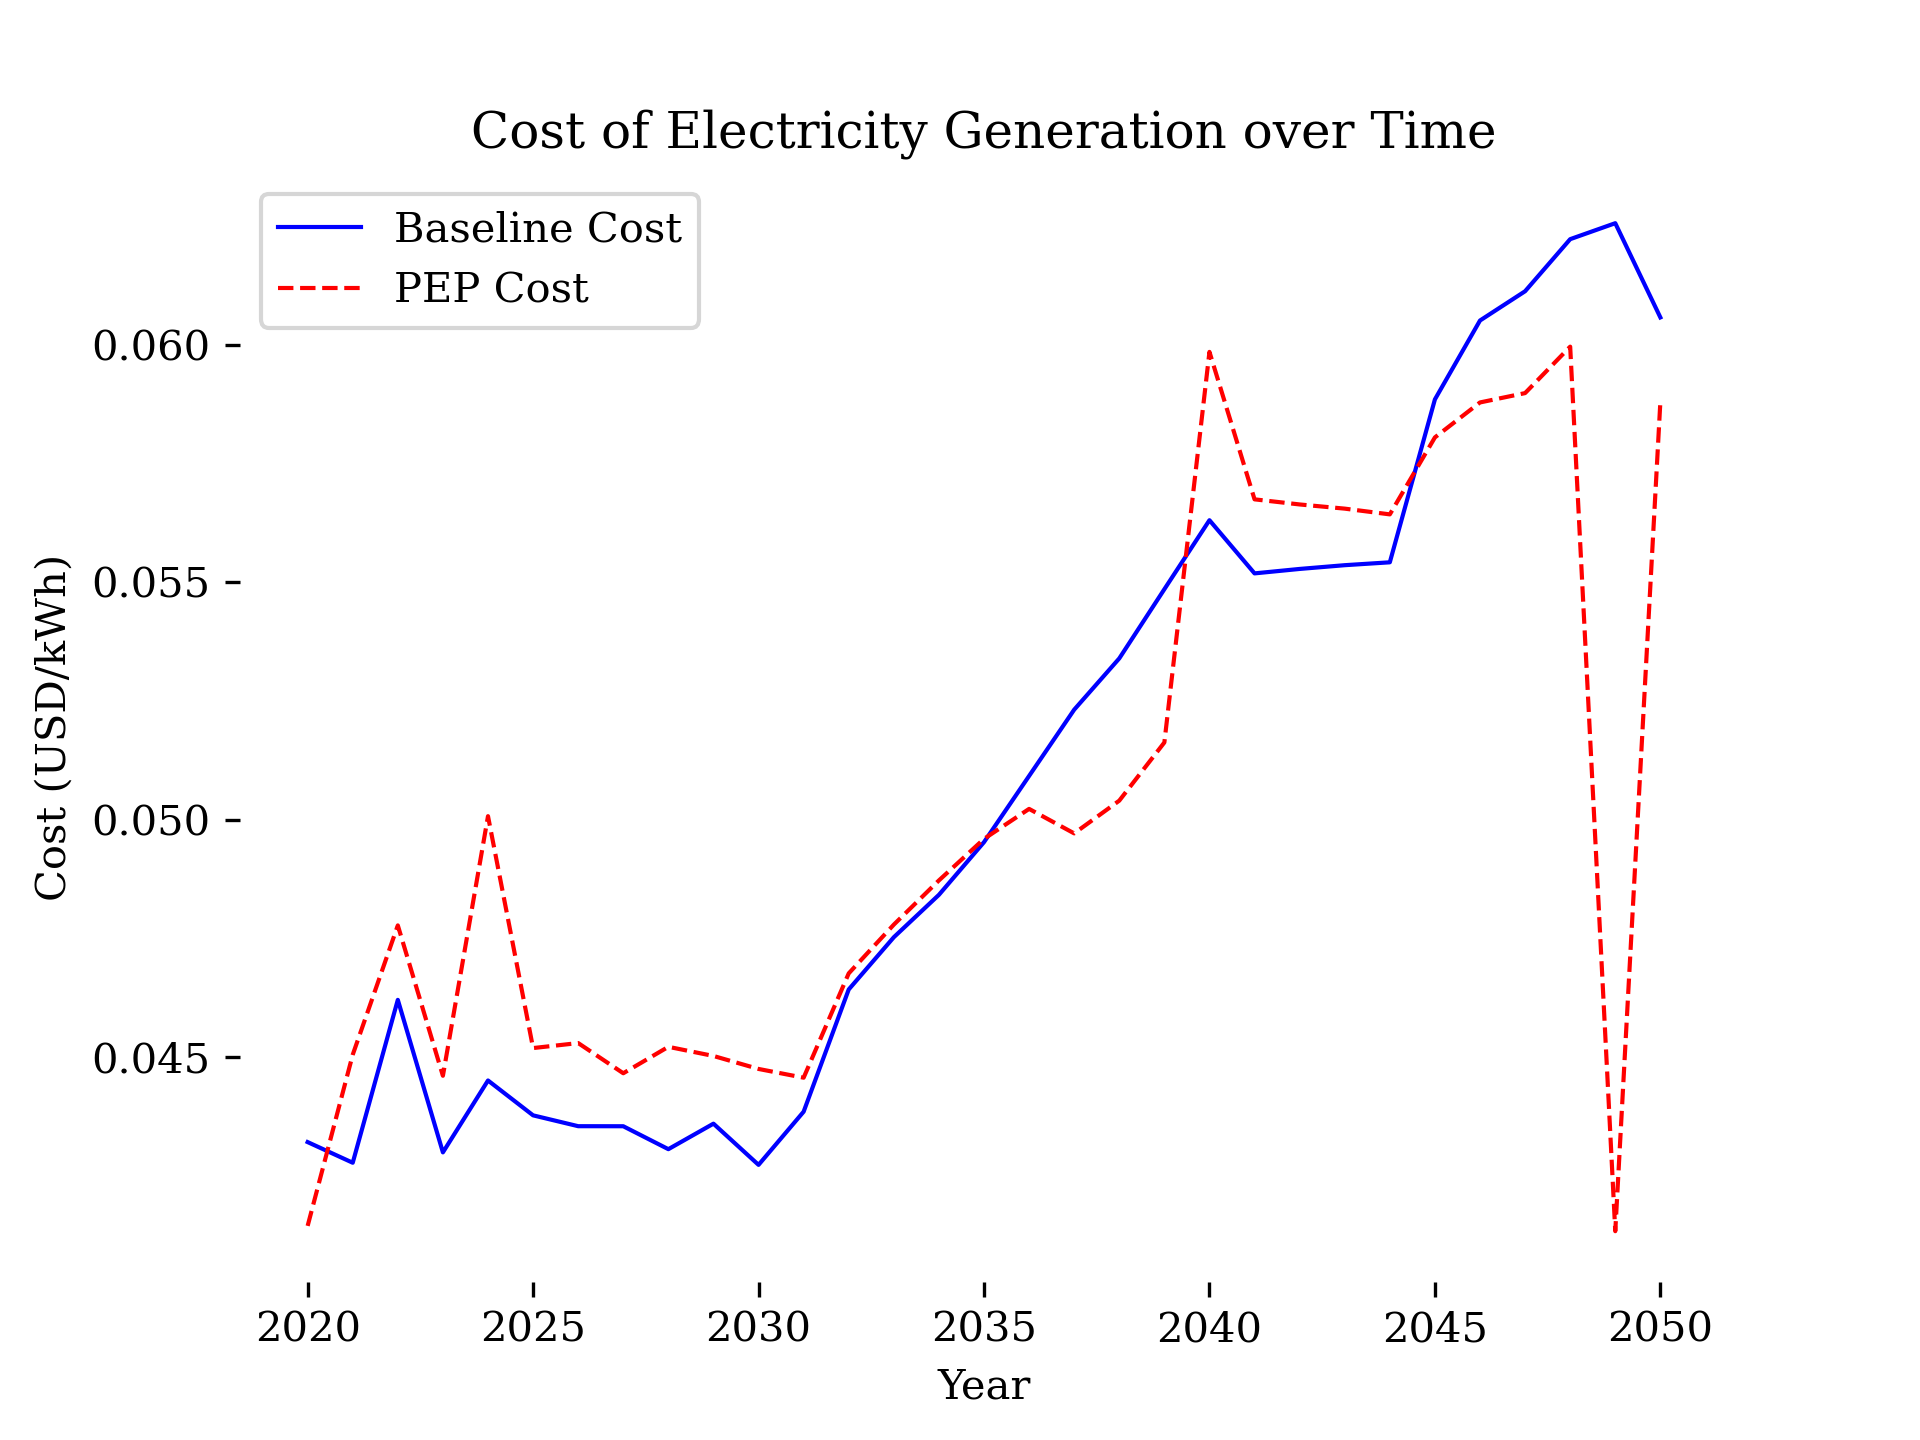
\includegraphics[height=0.75\textheight]{./images/PEP_Cost_of_Electricity_Generation.png}
  \end{figure}
\end{frame}

\begin{frame}
  \frametitle{OG-PHL: Energy Sector TFP over Time}
  \begin{figure}[htb]\centering
    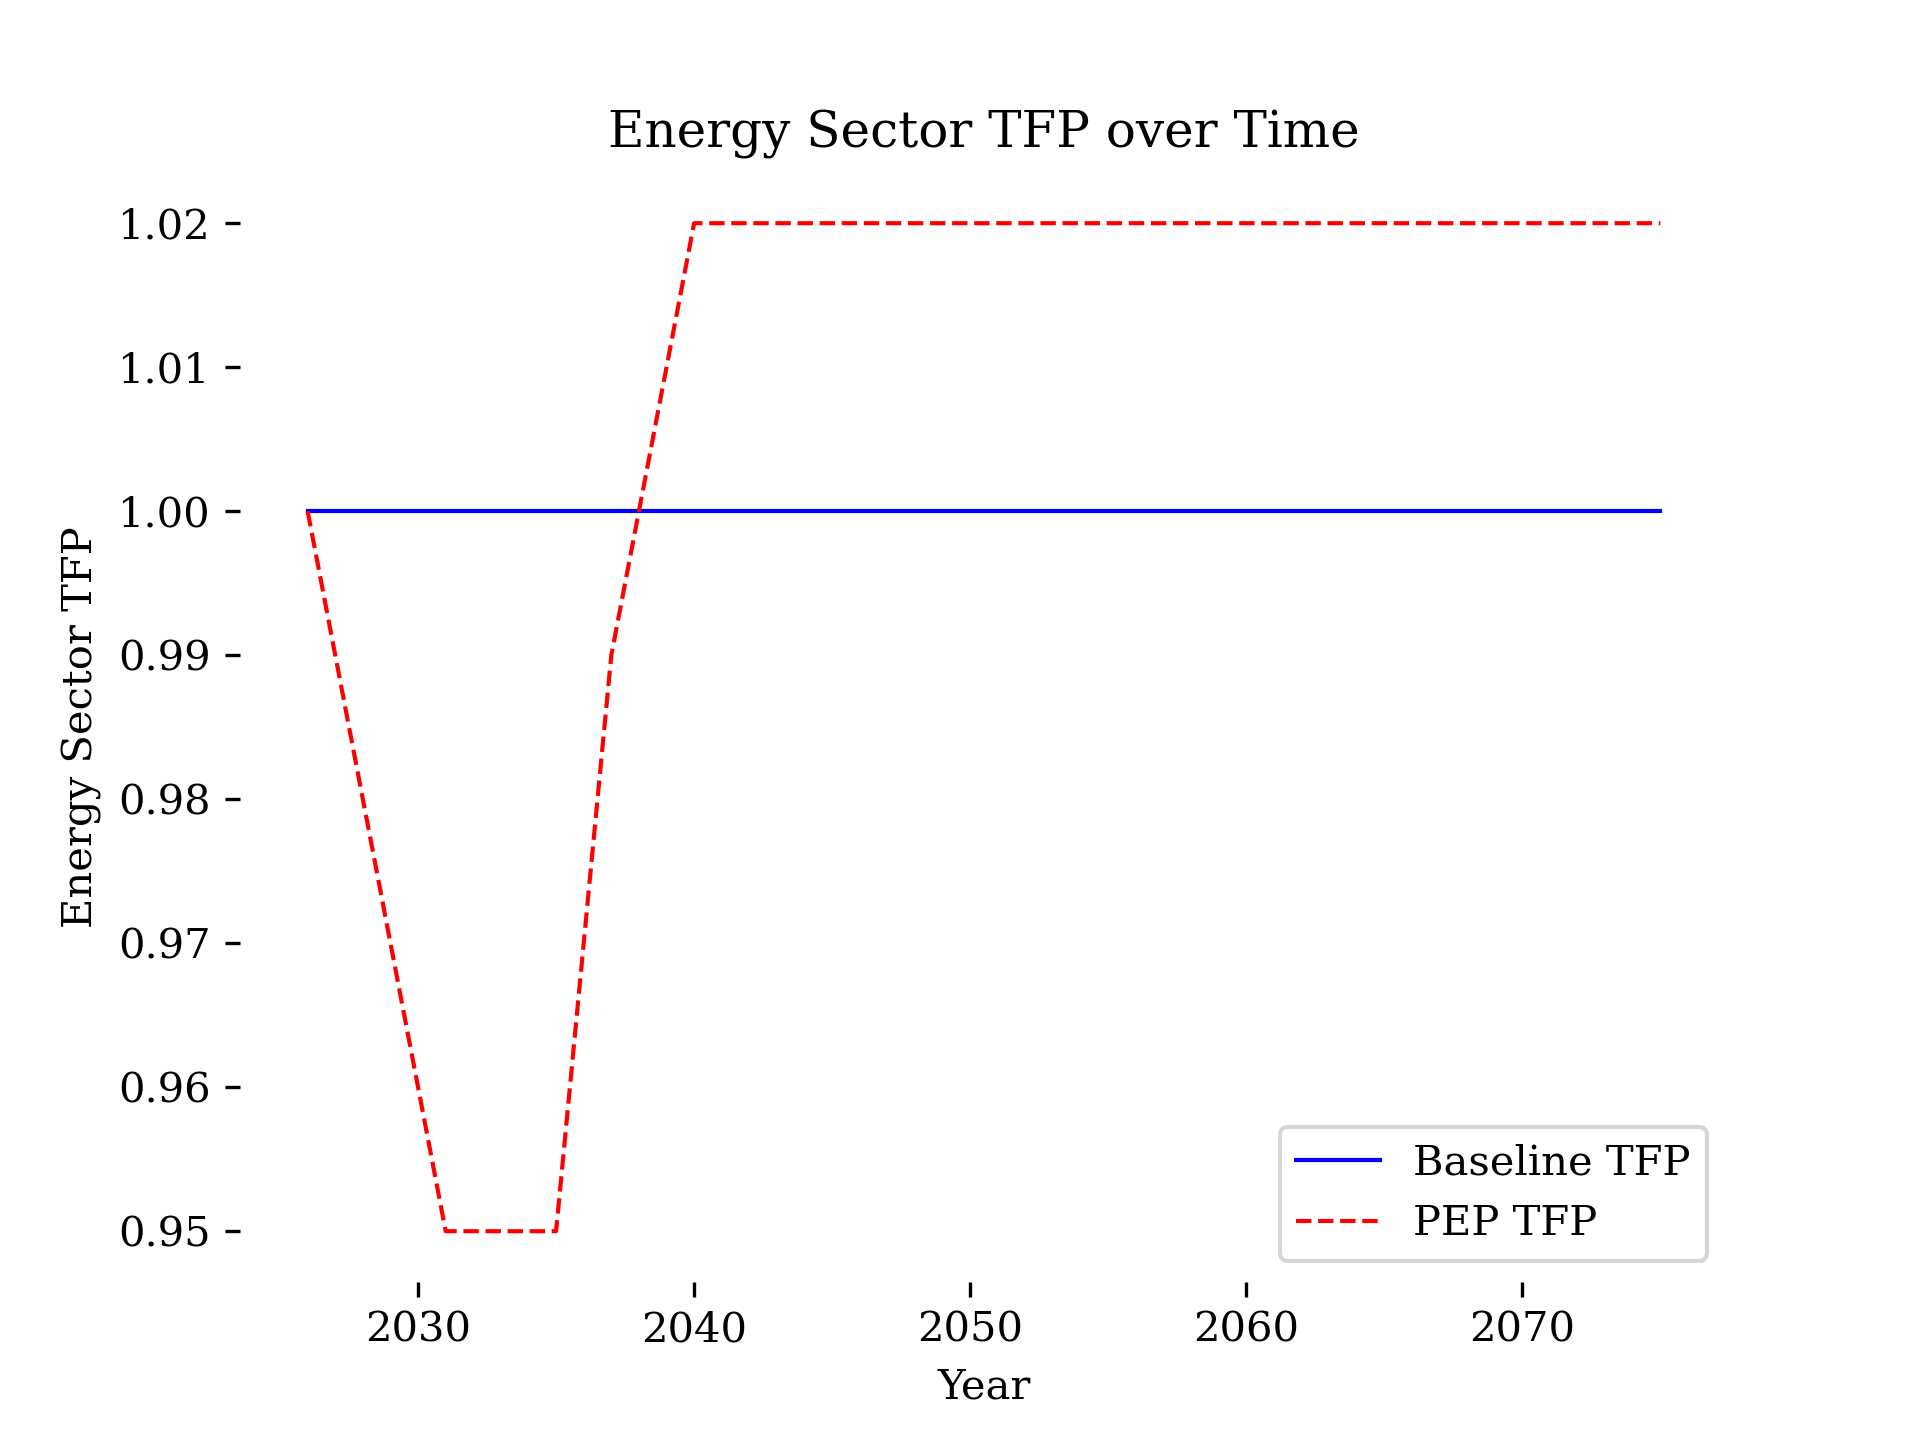
\includegraphics[height=0.75\textheight]{./images/PEP_Energy_Sector_TFP.png}
  \end{figure}
\end{frame}



\begin{frame}
  \frametitle{PEP23 Investments}
  \begin{itemize}
    \item PEP23 estimates total investments of 19.6-27.8 trillion PHP over 2023-2050
    \item This includes both government and private investments
    \item Government investments (both direct and via incentives and partnerships) are about 10\% of this total
    \item For our OG-PHL simulation, we assume government investments of 2.6 trillion PHP, spread over 27 years
    \item Private investment in endogenous in OG-PHL
  \end{itemize}
\end{frame}

\begin{frame}
  \frametitle{CLEWs: Annualized Investments over Time}

  \begin{figure}[htb]\centering
    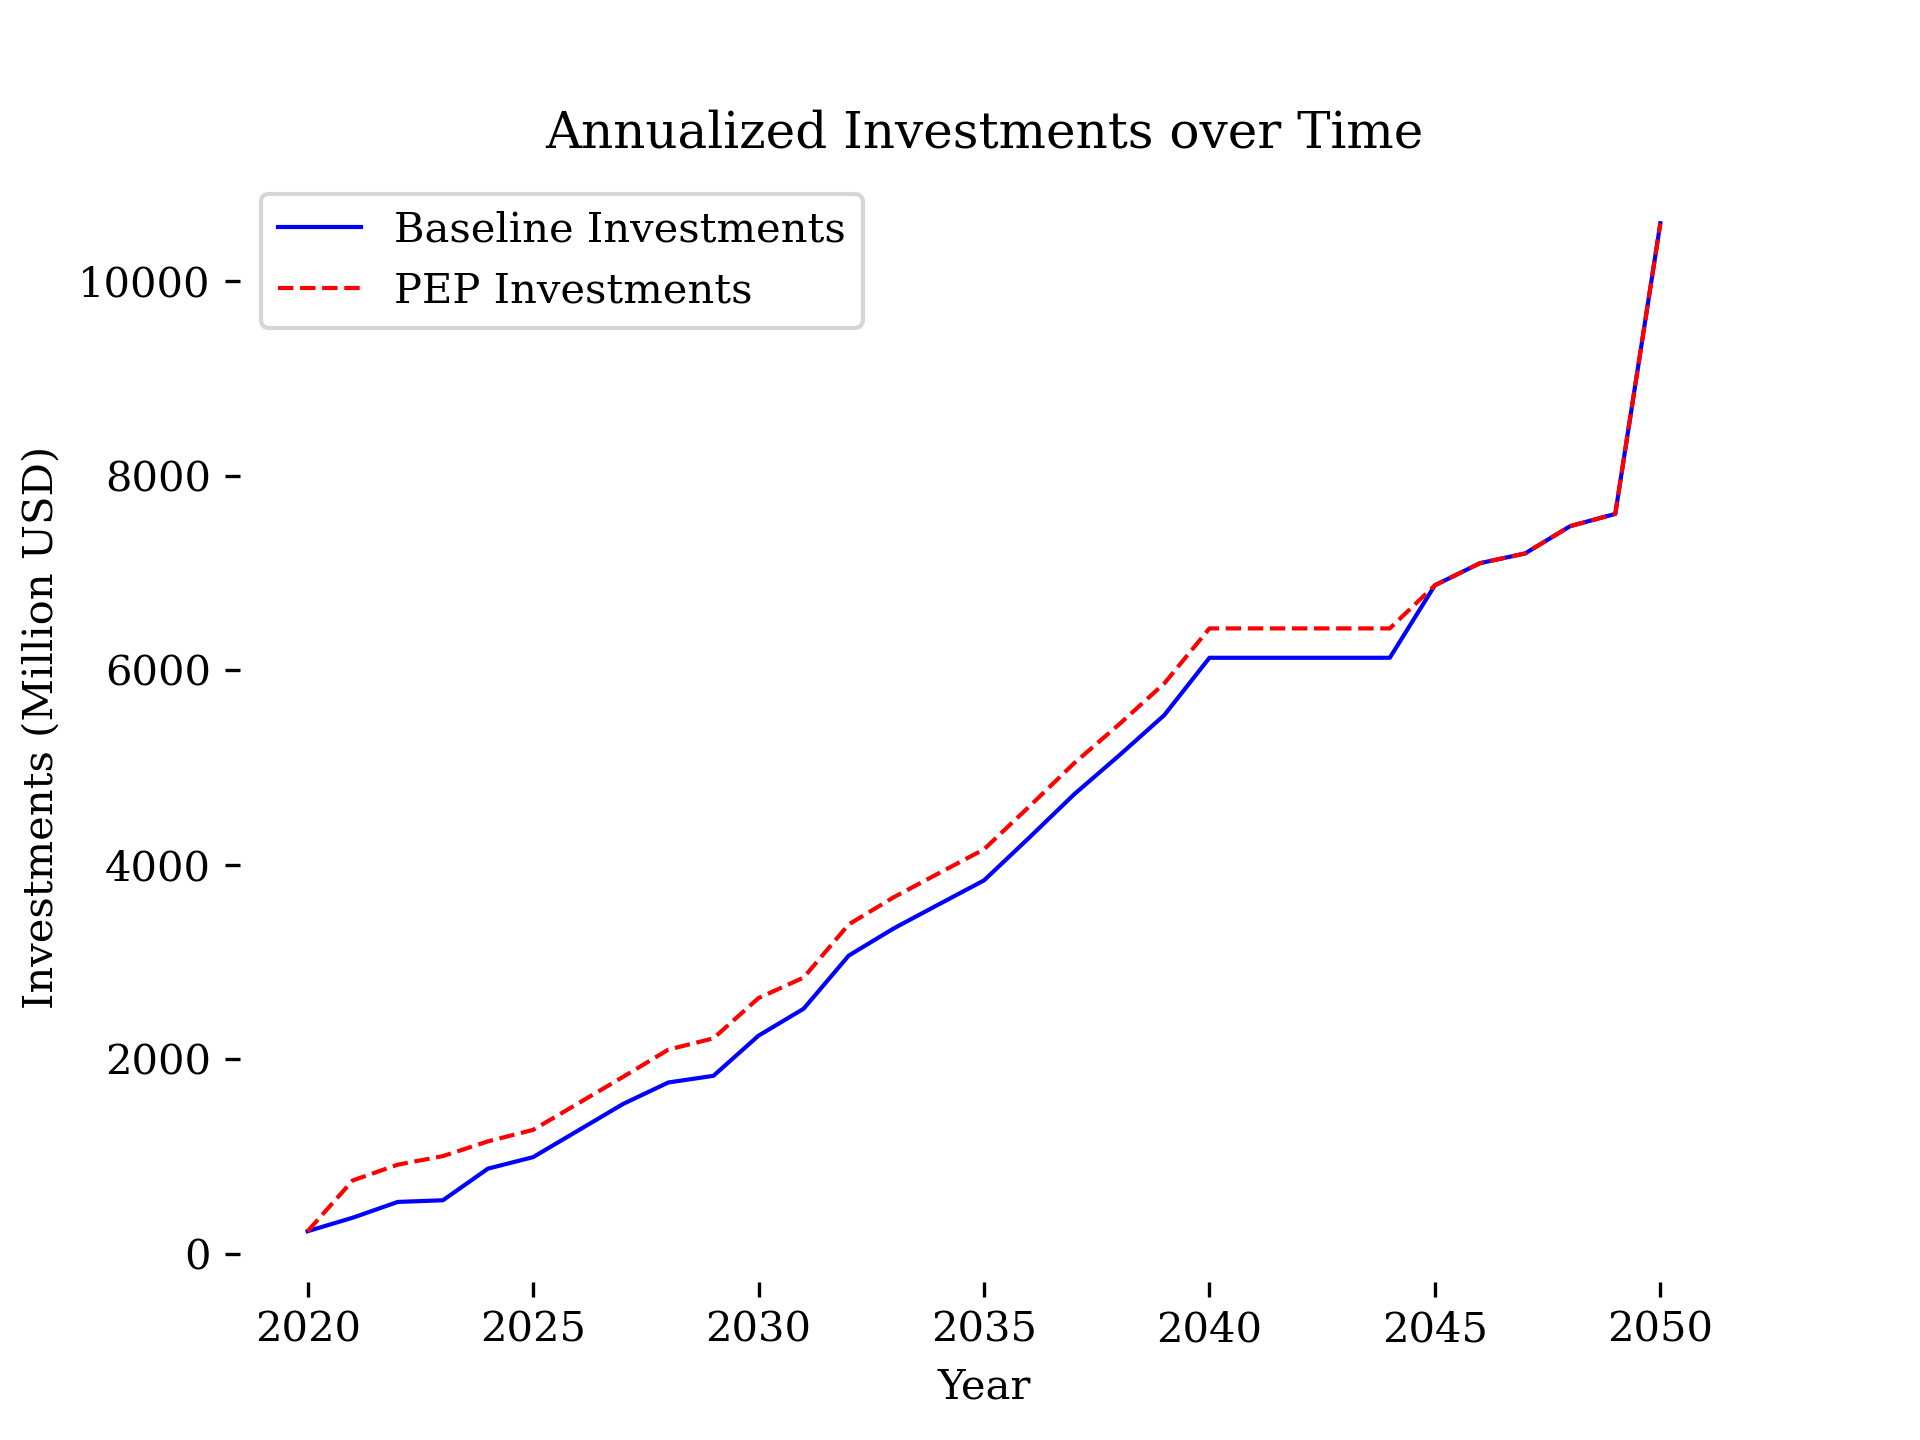
\includegraphics[height=0.75\textheight]{./images/PEP_Annualized_Investments.png}
  \end{figure}
\end{frame}


\begin{frame}
  \frametitle{OG-PHL: Government Spending over Time}

  \begin{figure}[htb]\centering
    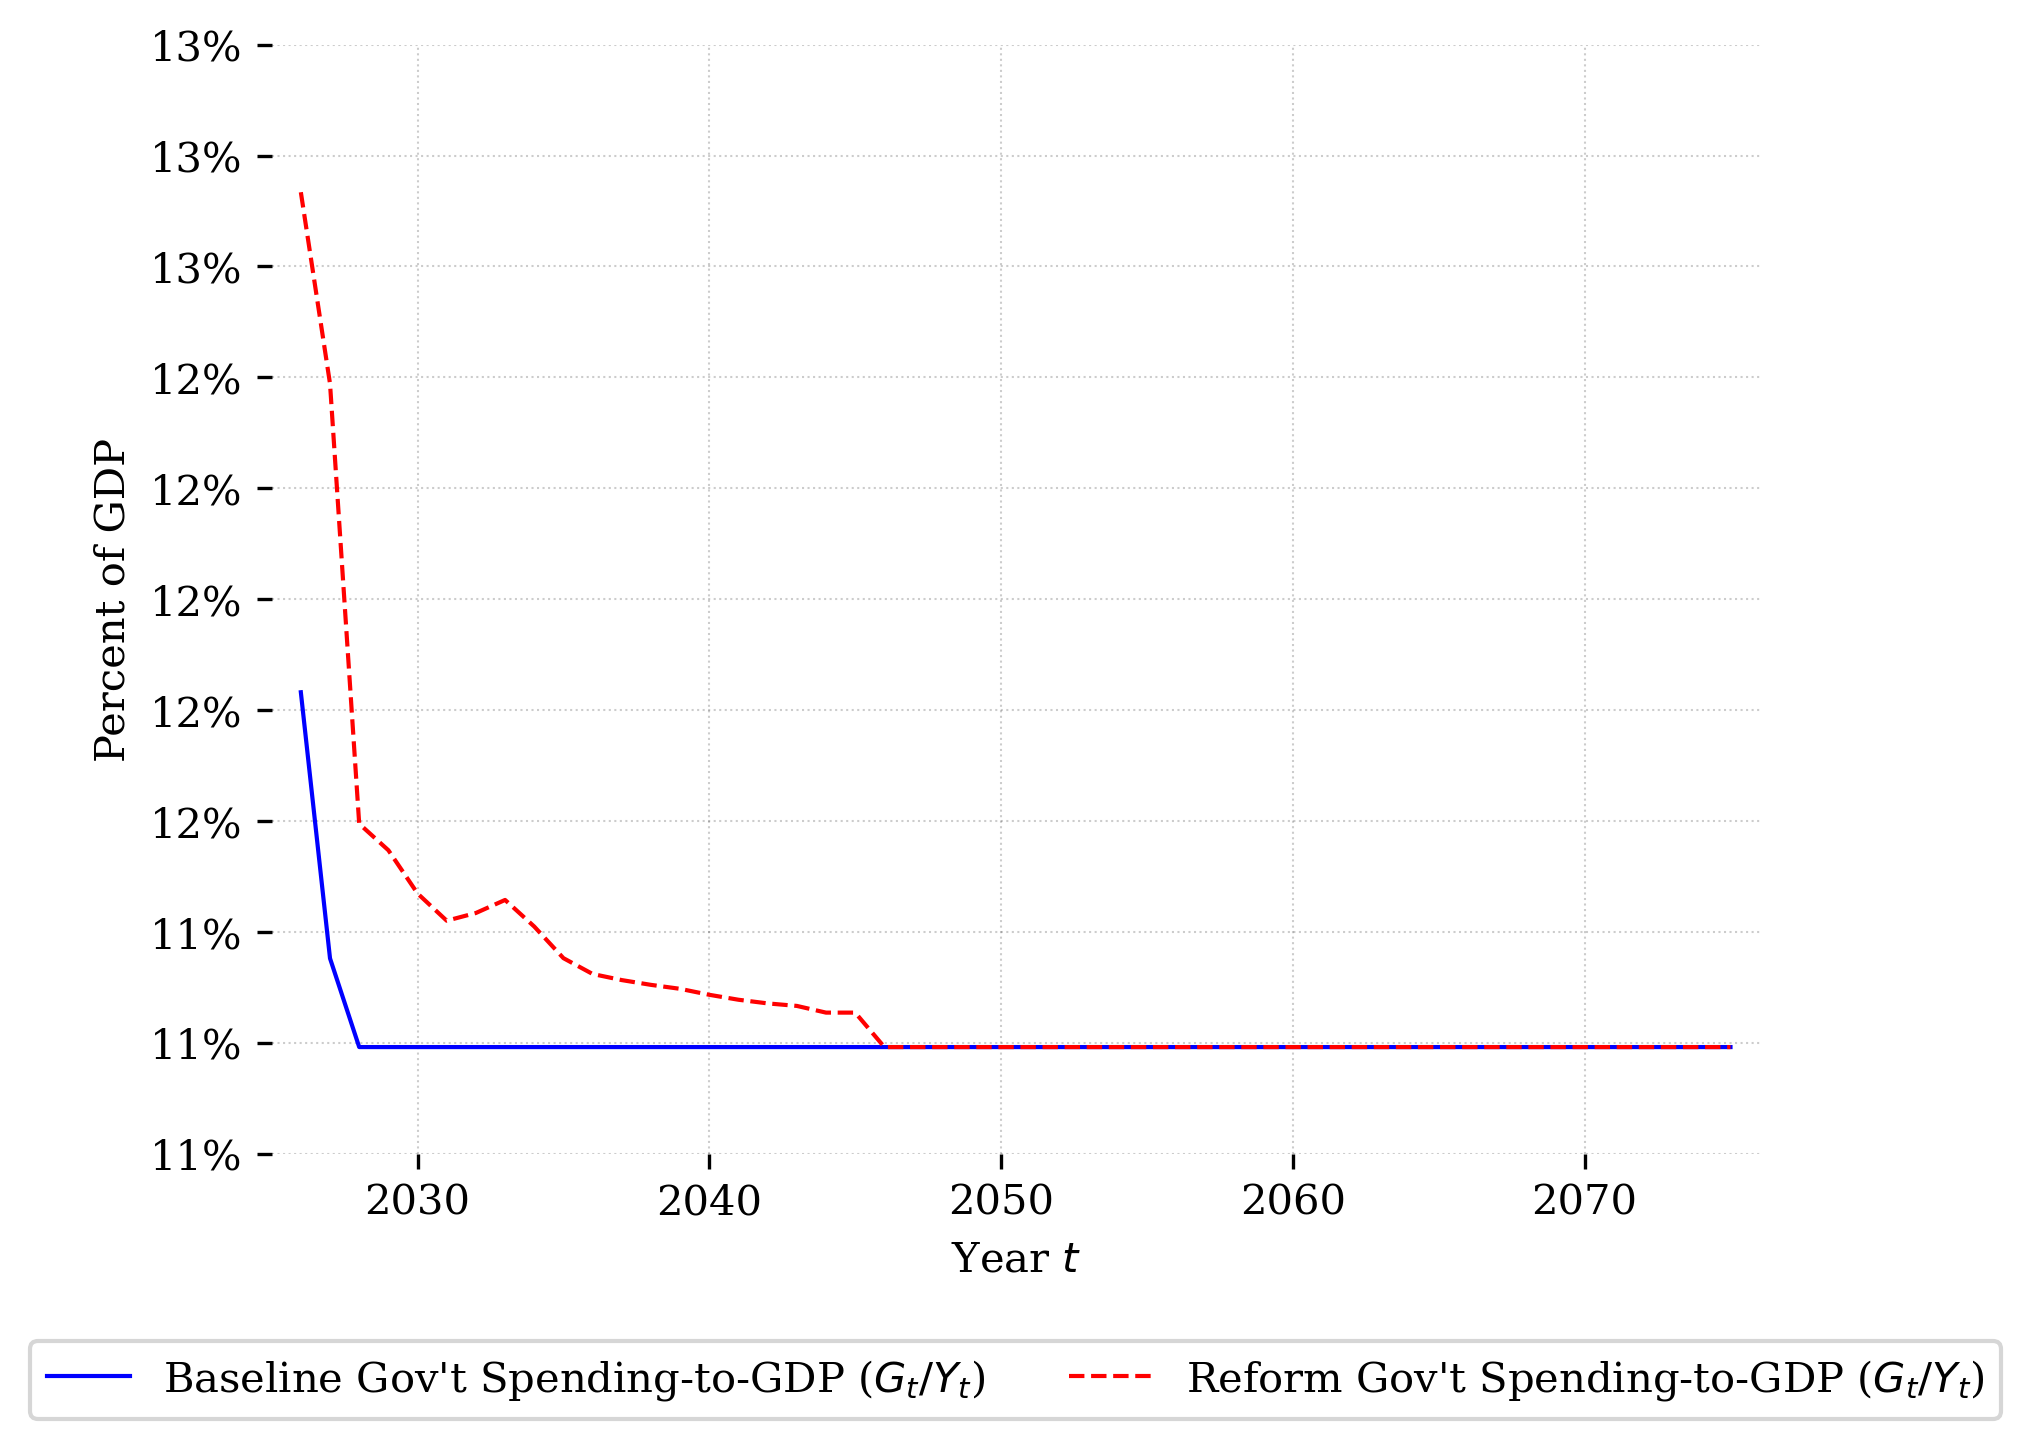
\includegraphics[height=0.75\textheight]{./images/PEP_G_over_Y.png}
  \end{figure}
\end{frame}



\section{Env. Outcomes}

\begin{frame}
  \frametitle{CLEWs: CO2 Emissions over Time}

  \begin{figure}[htb]\centering
    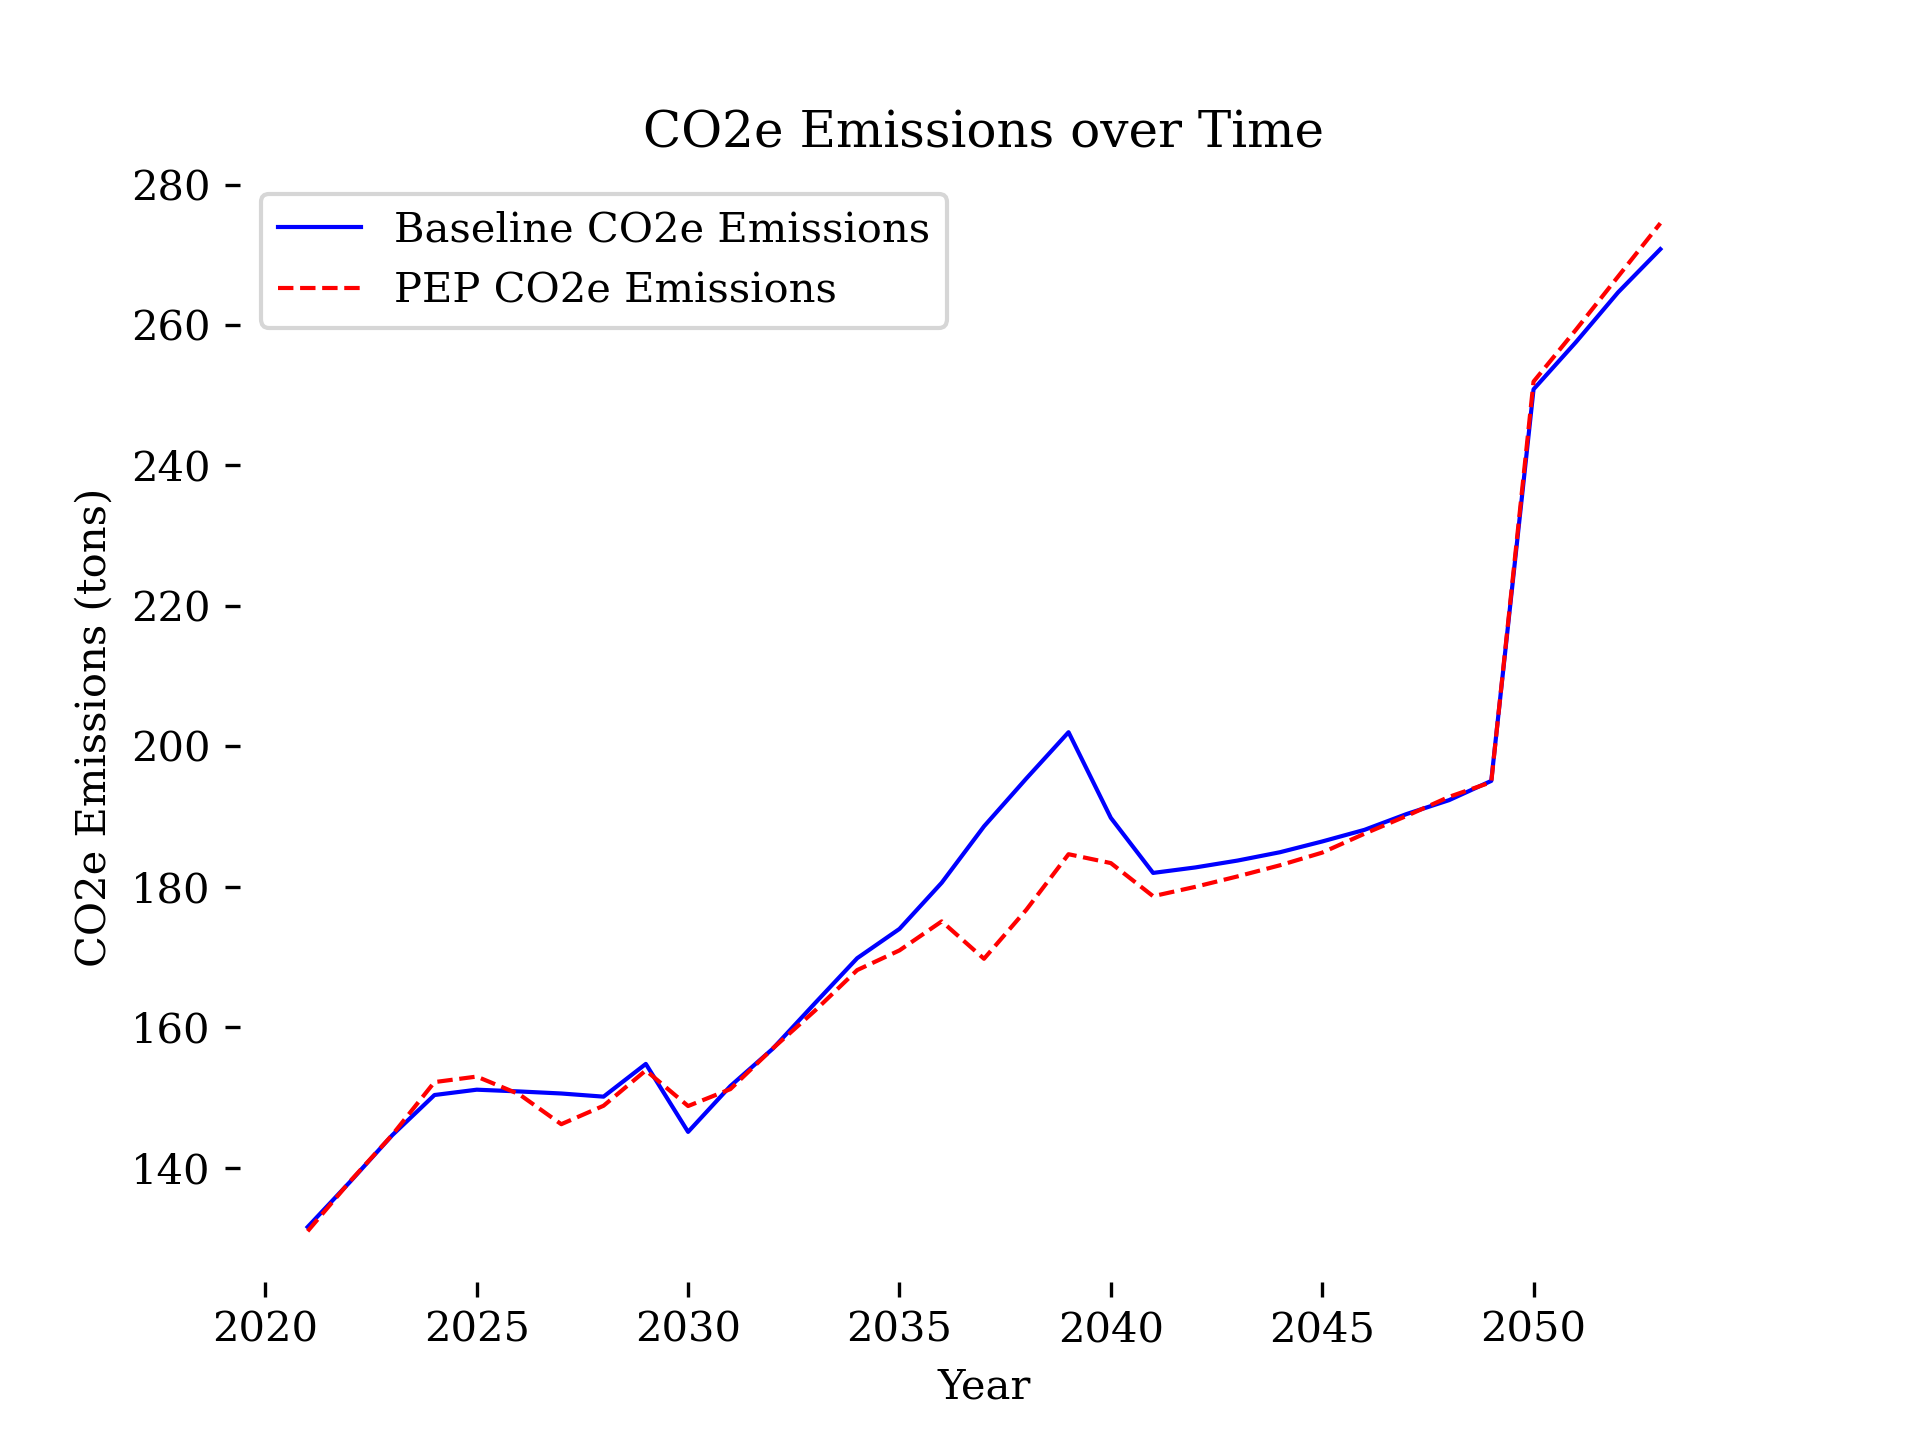
\includegraphics[height=0.75\textheight]{./images/PEP_CO2e_Emissions.png}
  \end{figure}
\end{frame}


\begin{frame}
  \frametitle{CLEWs: PM2.5 Concentration over Time}

  \begin{figure}[htb]\centering
    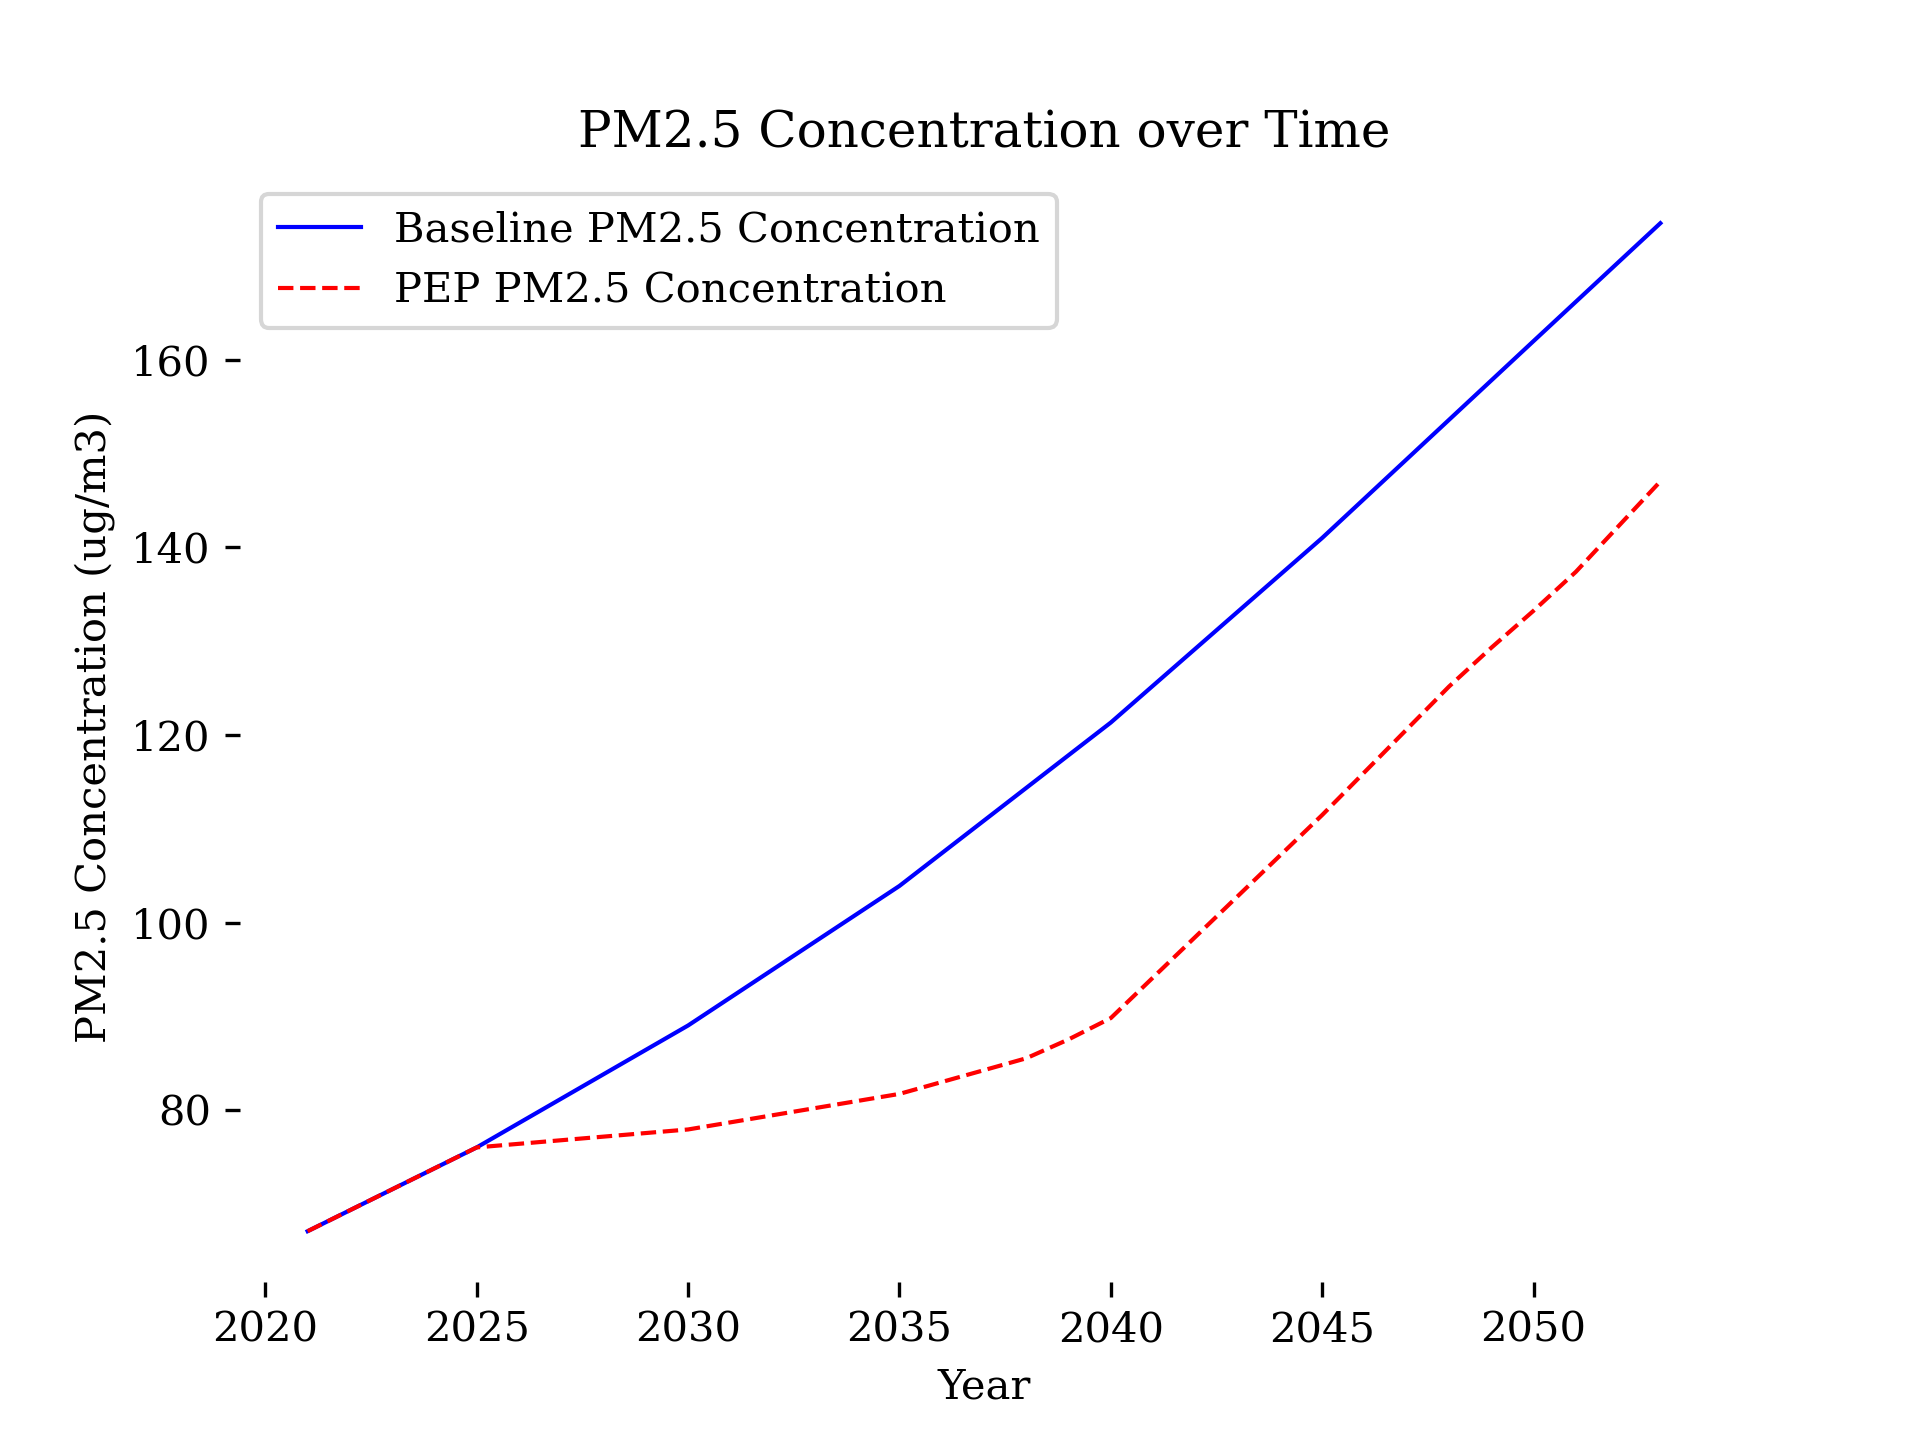
\includegraphics[height=0.75\textheight]{./images/PEP_PM2.5_Concentration.png}
  \end{figure}
\end{frame}


\section{Health Impacts}


\begin{frame}
  \frametitle{Mapping PM2.5 to Labor Productivity}

  \begin{itemize}
    \item There are strong links in the literature between air pollution (PM2.5) and economic outcomes, including labor productivity
    \item He, Liu, and Salvo (\emph{AEJ: Applied}, 2019) find that a \textbf{50\% decline in PM2.5 reduces productivity by 3\%}
    \item We use this mapping to adjust key productivity parameters in OG-PHL:
      \begin{itemize}
        \item Ability profiles
        \item Disutility of labor parameters
      \end{itemize}
    \item CLEWS finds a 15\% reduction in PM2.5 under PEP scenario, leading to a 0.9\% increase in productivity
  \end{itemize}
\end{frame}

\begin{frame}
  \frametitle{Ability Profiles in Baseline and PEP}

  \begin{figure}[htb]\centering
    
\includegraphics[height=0.75\textheight]{./images/ability_profiles.png}
  \end{figure}
\end{frame}


\begin{frame}
  \frametitle{Disutility of Labor in Baseline and PEP}

  \begin{figure}[htb]\centering
    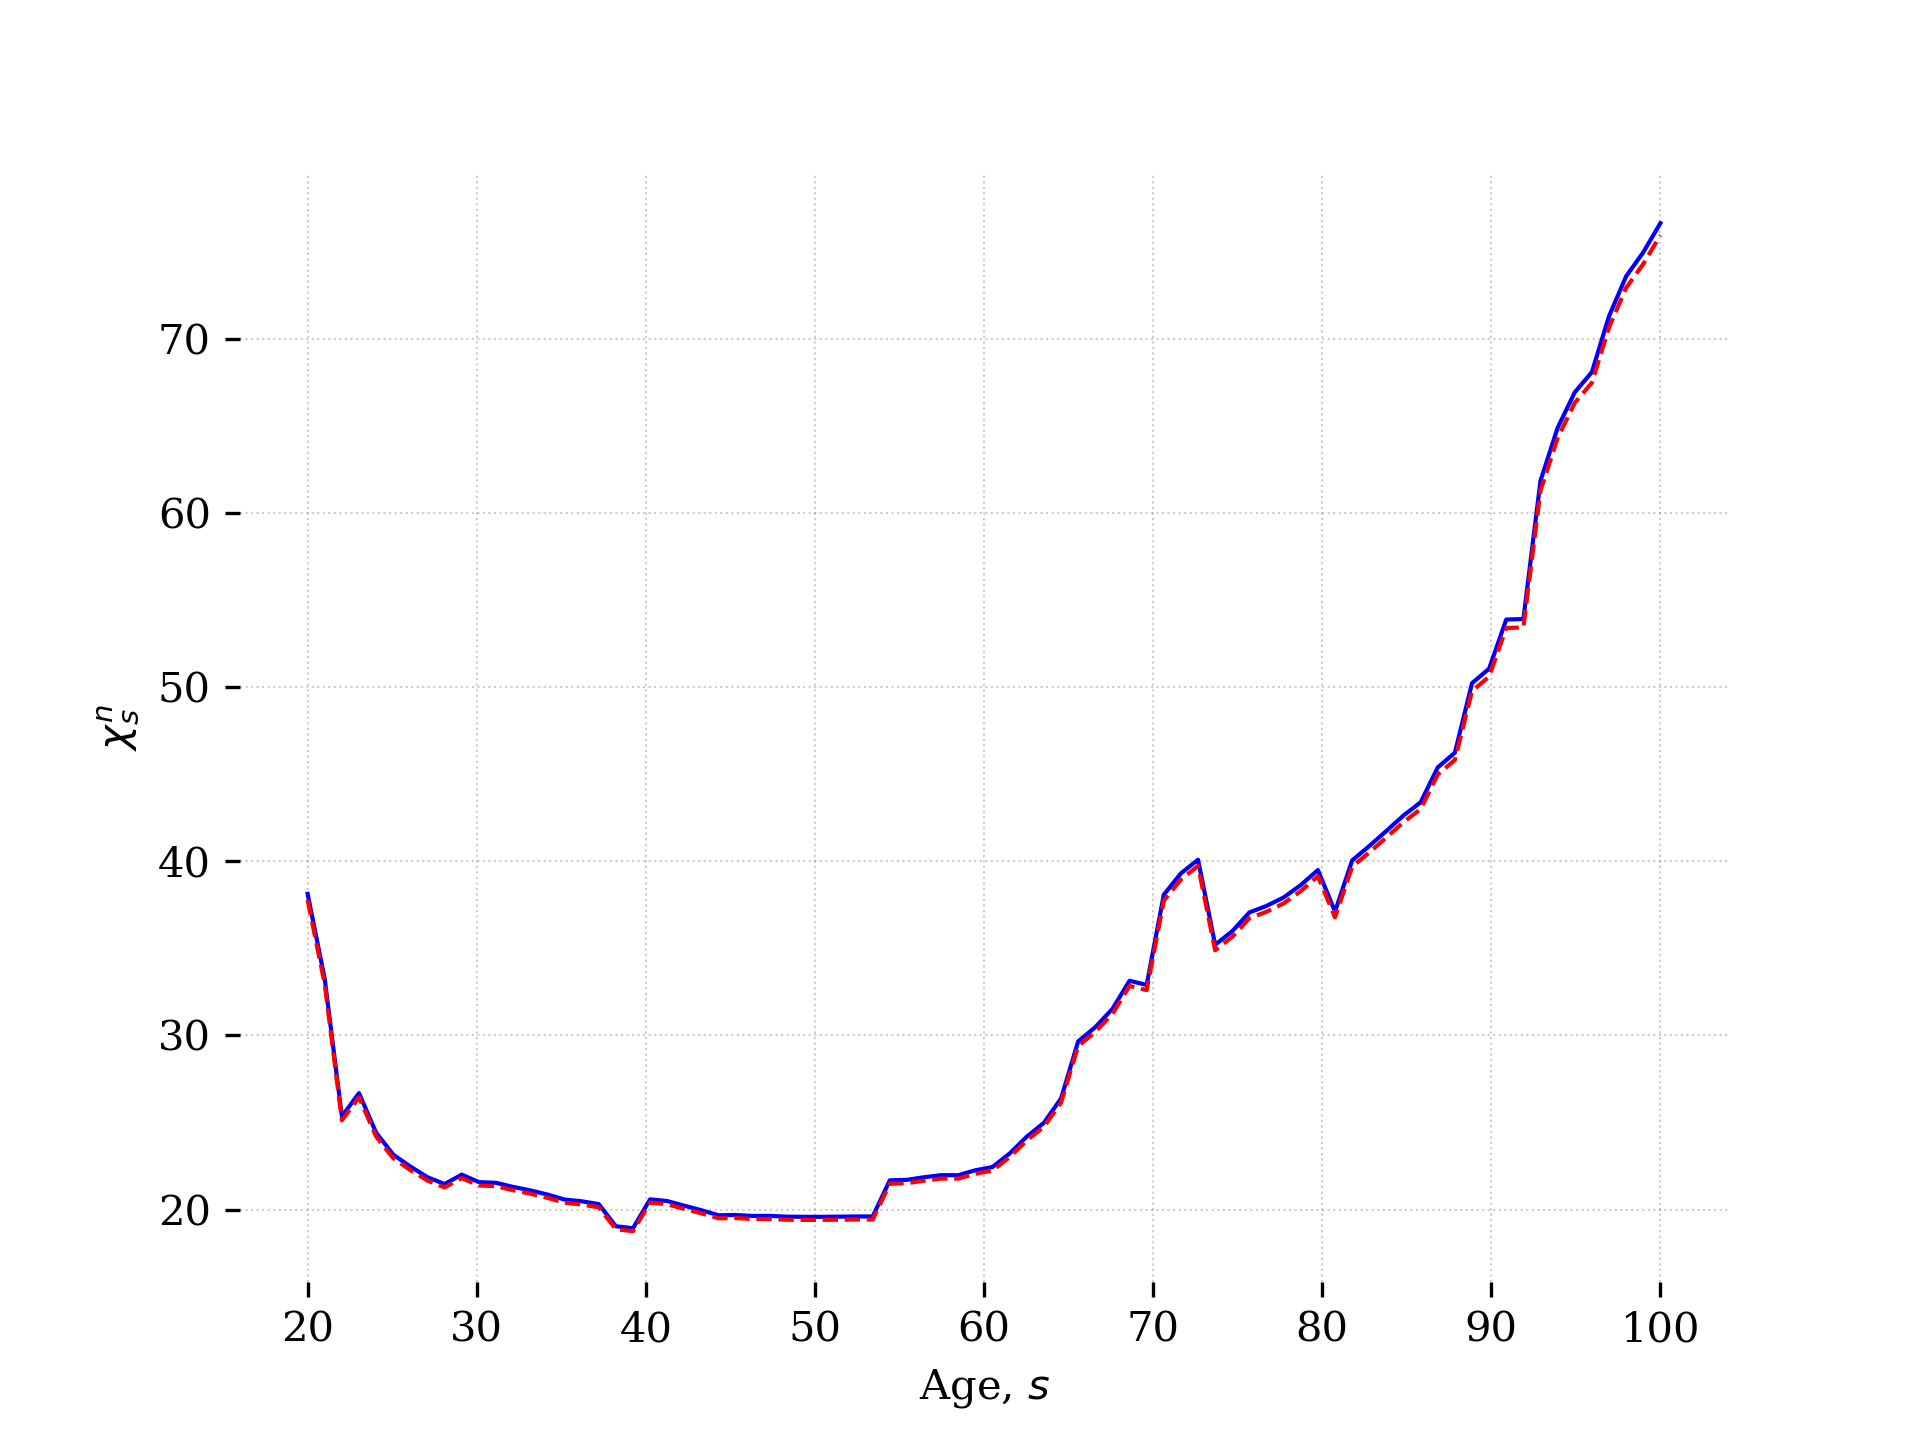
\includegraphics[height=0.75\textheight]{./images/chi_n_values.png}
  \end{figure}
\end{frame}


\begin{frame}
  \frametitle{Mapping PM2.5 to Mortality}

  \begin{itemize}
    \item A substantial scientific literature establishing a link between air pollution (PM2.5) and mortality:
      \begin{itemize}
        \item Pope et al. (\emph{Air Quality, Atmosphere, and Health}, 2017): 6-34\% change in mortality per  10$\mu$g/m$^3$ change in PM2.5
        \item Kim et al. (\emph{Environmental Health}, 2021):  10$\mu$g/m$^3$ increase in in PM2.5 lowers life expectancy by 0.7-0.9 years
        \item Puett et al. (\emph{Environmental Health Perspectives}, 2009): 10$\mu$g/m$^3$ increase in PM2.5 leads to 4\% increase in all-cause mortality risk
      \end{itemize}
    \item We take the estimates of Pope et al. (\emph{Air Quality, Atmosphere, and Health}, 2017) to map PM2.5 concentrations to mortality risk
    \item The decrease in PM2.5 under the PEP scenario is about 10$\mu$g/m$^3$, which we map to a conservative 4\% decrease in mortality risk
  \end{itemize}
\end{frame}

\begin{frame}
  \frametitle{Mortality Baseline and PEP}

  \begin{figure}[htb]\centering
    
\includegraphics[height=0.75\textheight]{./images/survival_rates.png}
  \end{figure}
\end{frame}


\begin{frame}
  \frametitle{Annual Deaths over Time}

  \begin{figure}[htb]\centering
    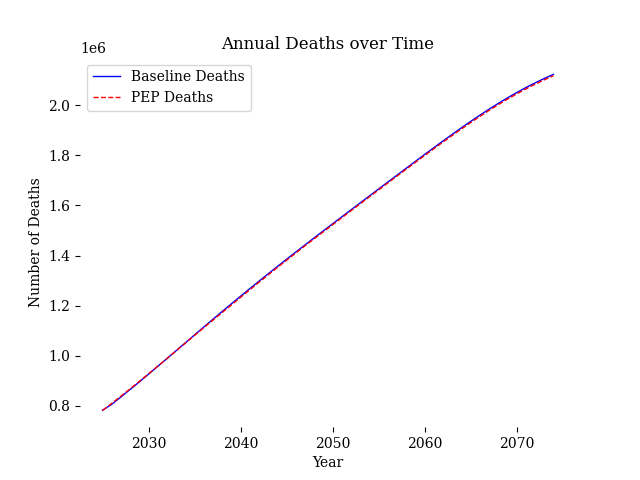
\includegraphics[height=0.75\textheight]{./images/PEP_Annual_Deaths.png}
  \end{figure}
\end{frame}


\begin{frame}
  \frametitle{Cumulative Deaths Averted over Time}

  \begin{figure}[htb]\centering
    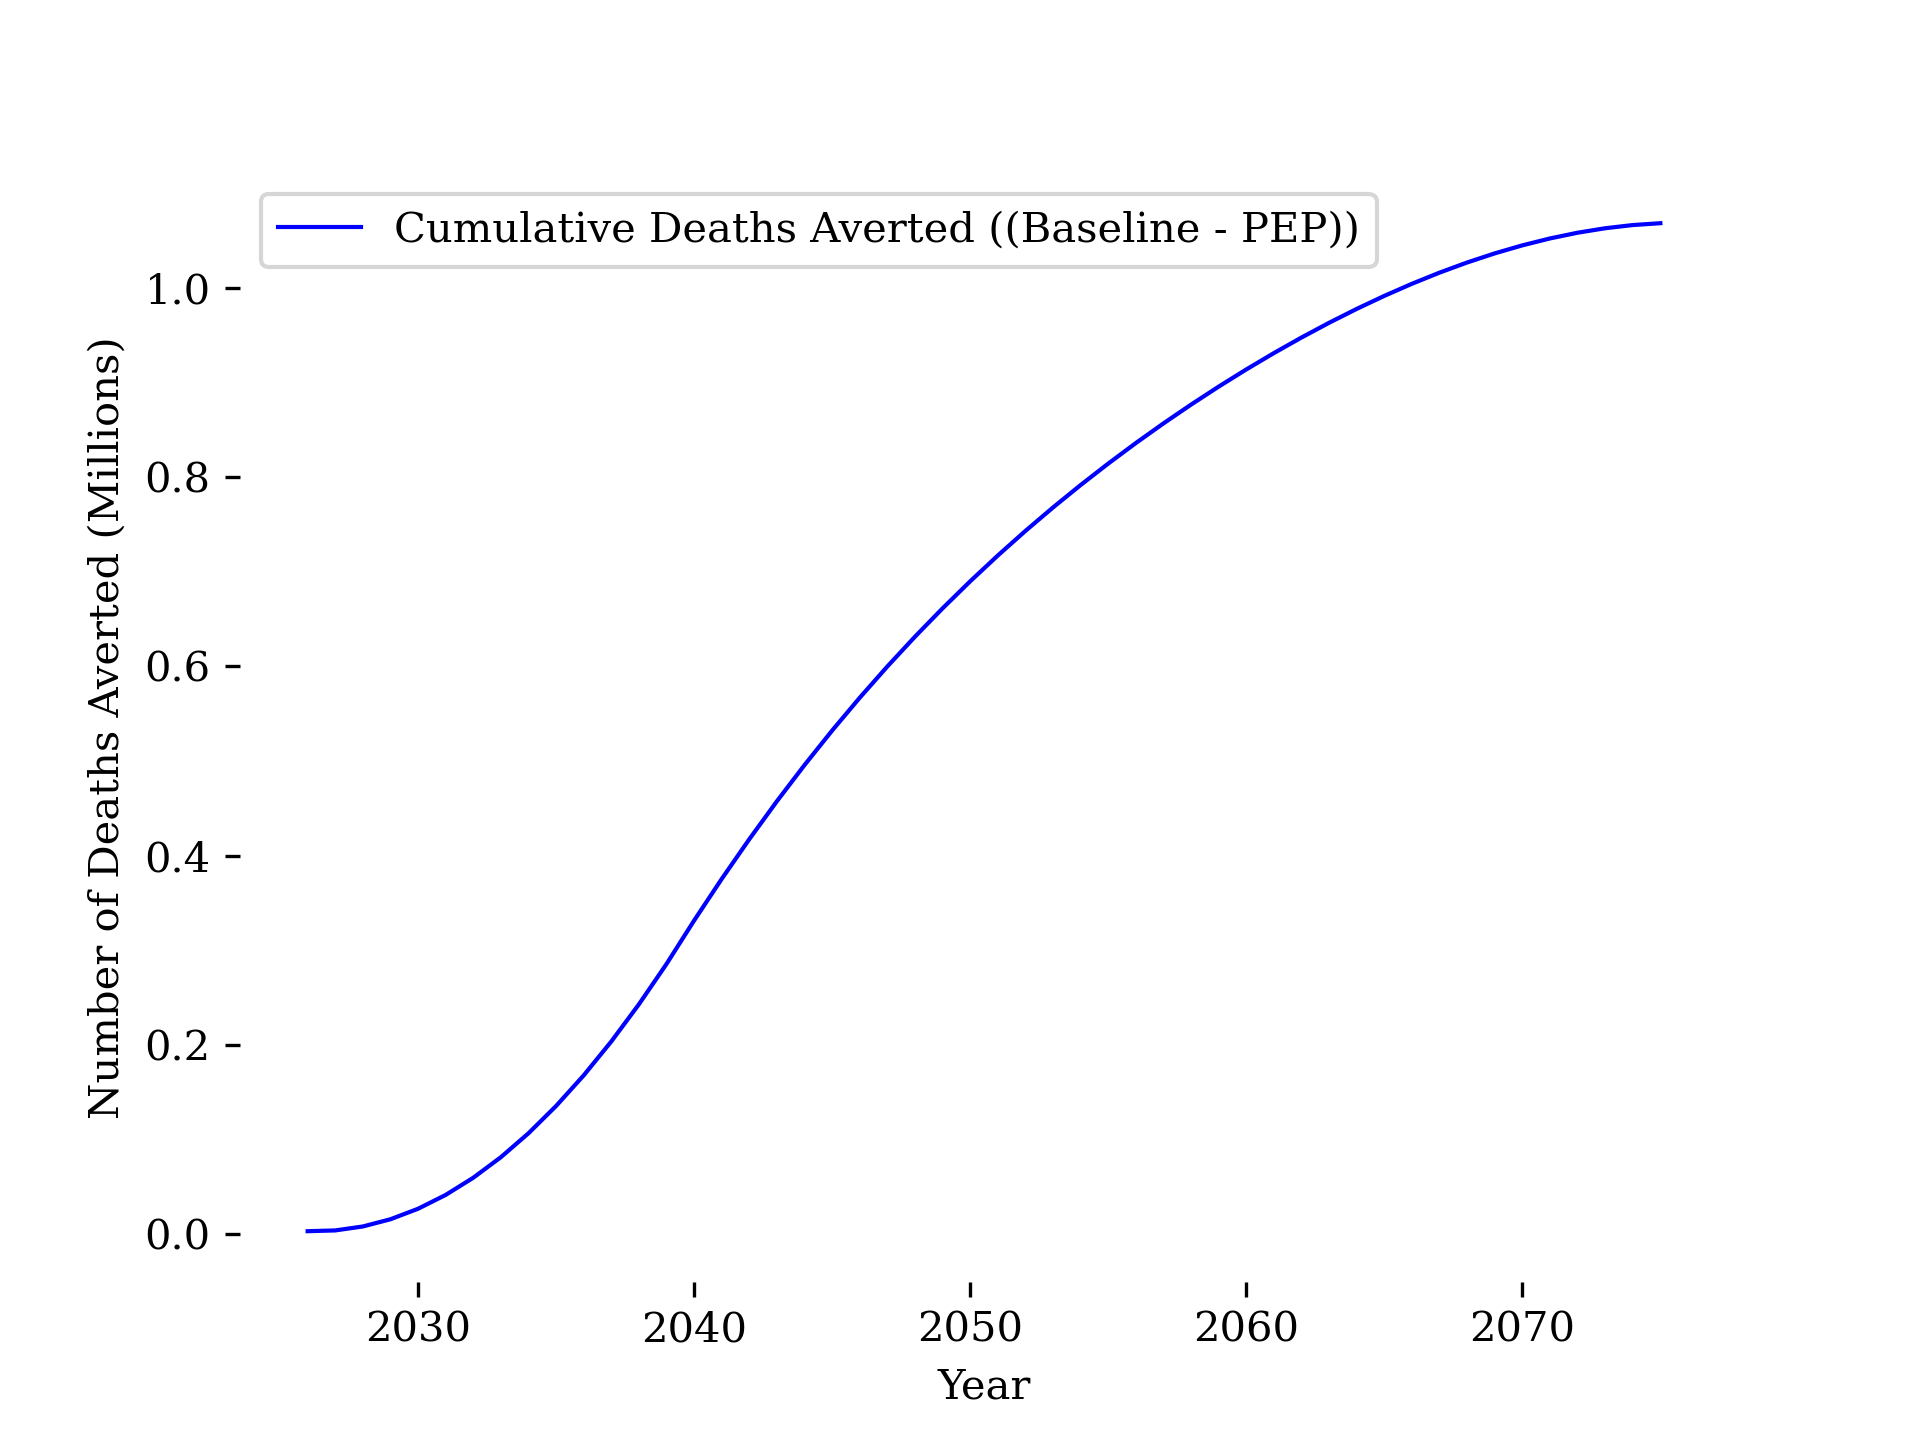
\includegraphics[height=0.75\textheight]{./images/PEP_Cumulative_Deaths_Averted.png}
  \end{figure}
\end{frame}


\begin{frame}
  \frametitle{Labor Supply over Time}

  \begin{figure}[htb]\centering
    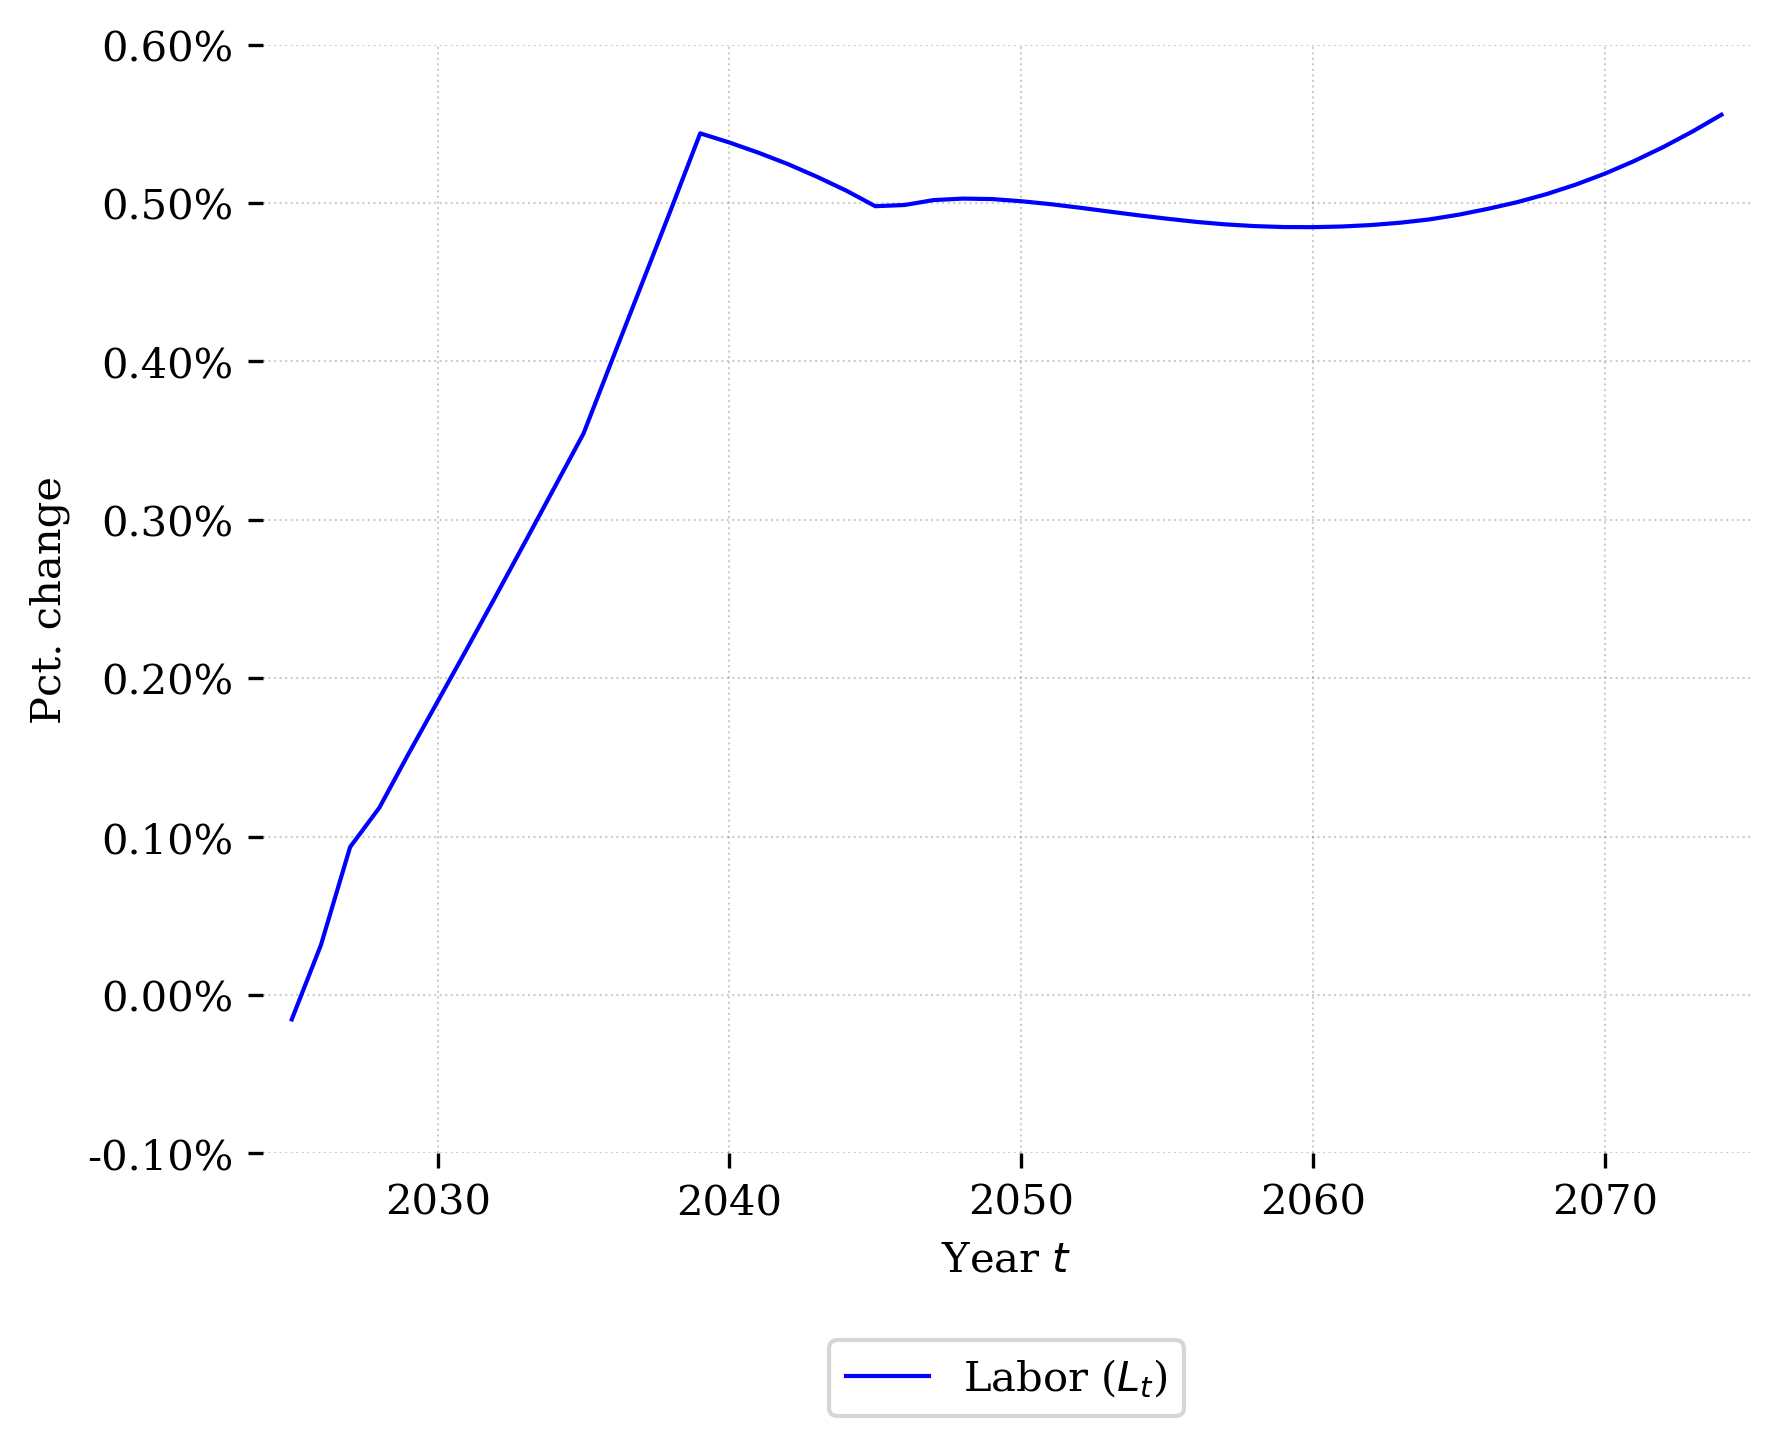
\includegraphics[height=0.75\textheight]{./images/PEP_deaths_over_time.png}
  \end{figure}
\end{frame}


\section{Macro Impacts}

\begin{frame}
  \frametitle{Aggregate Variables over Time}

  \begin{itemize}
    \item Percentage changes in capital (K), output (Y), consumption (C), and labor (L)
  \end{itemize}

  \begin{figure}[htb]\centering
    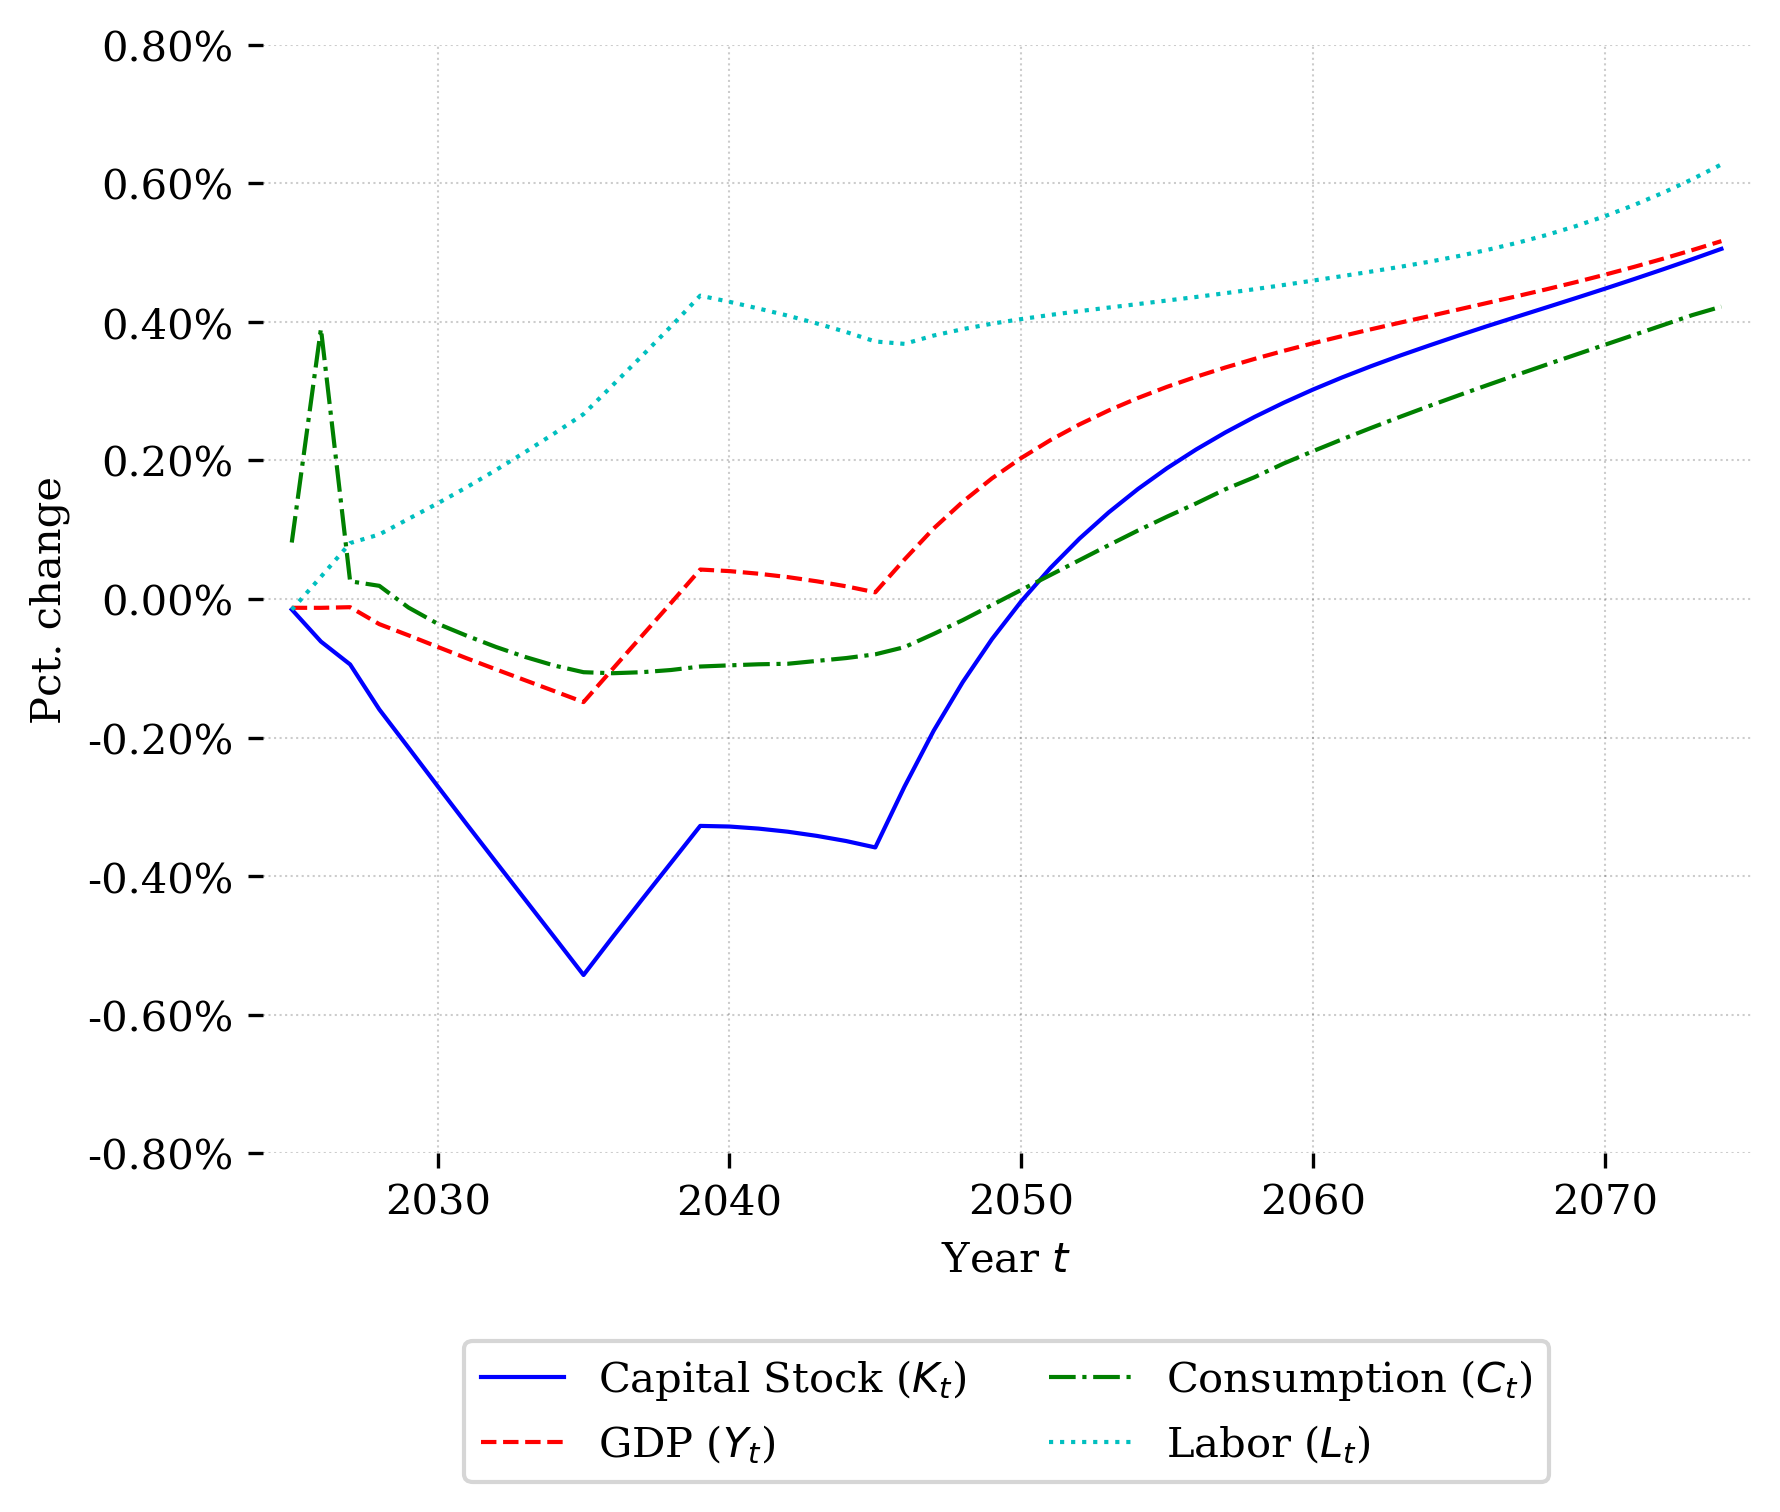
\includegraphics[height=0.65\textheight]{./images/PEP_agg_over_time.png}
  \end{figure}
\end{frame}

\begin{frame}
  \frametitle{Long Run Effects on GDP}
\begin{table}
% \caption{NPV of GDP Effects under Different Discount Rates}
\label{tab:PEP_NPV_GDP_Effects_Table}
\begin{tabular}{cc}
\hline
\hline
 Discount Rate & NPV of GDP Increase \\
   & (Trillions of PHP) \\
\hline
 1\% & 5,073.030 \\
 2\% & 2,216.387 \\
 3\% & 998.952 \\
 4\% & 466.805 \\
 5\% & 227.508 \\
\hline
\hline
\end{tabular}
\end{table}

Note: PEP23 Estimate of costs: ~26-42 Trillion PHP
\end{frame}

\begin{frame}
  \frametitle{Debt-to-GDP Ratio over Time}

  \begin{figure}[htb]\centering
    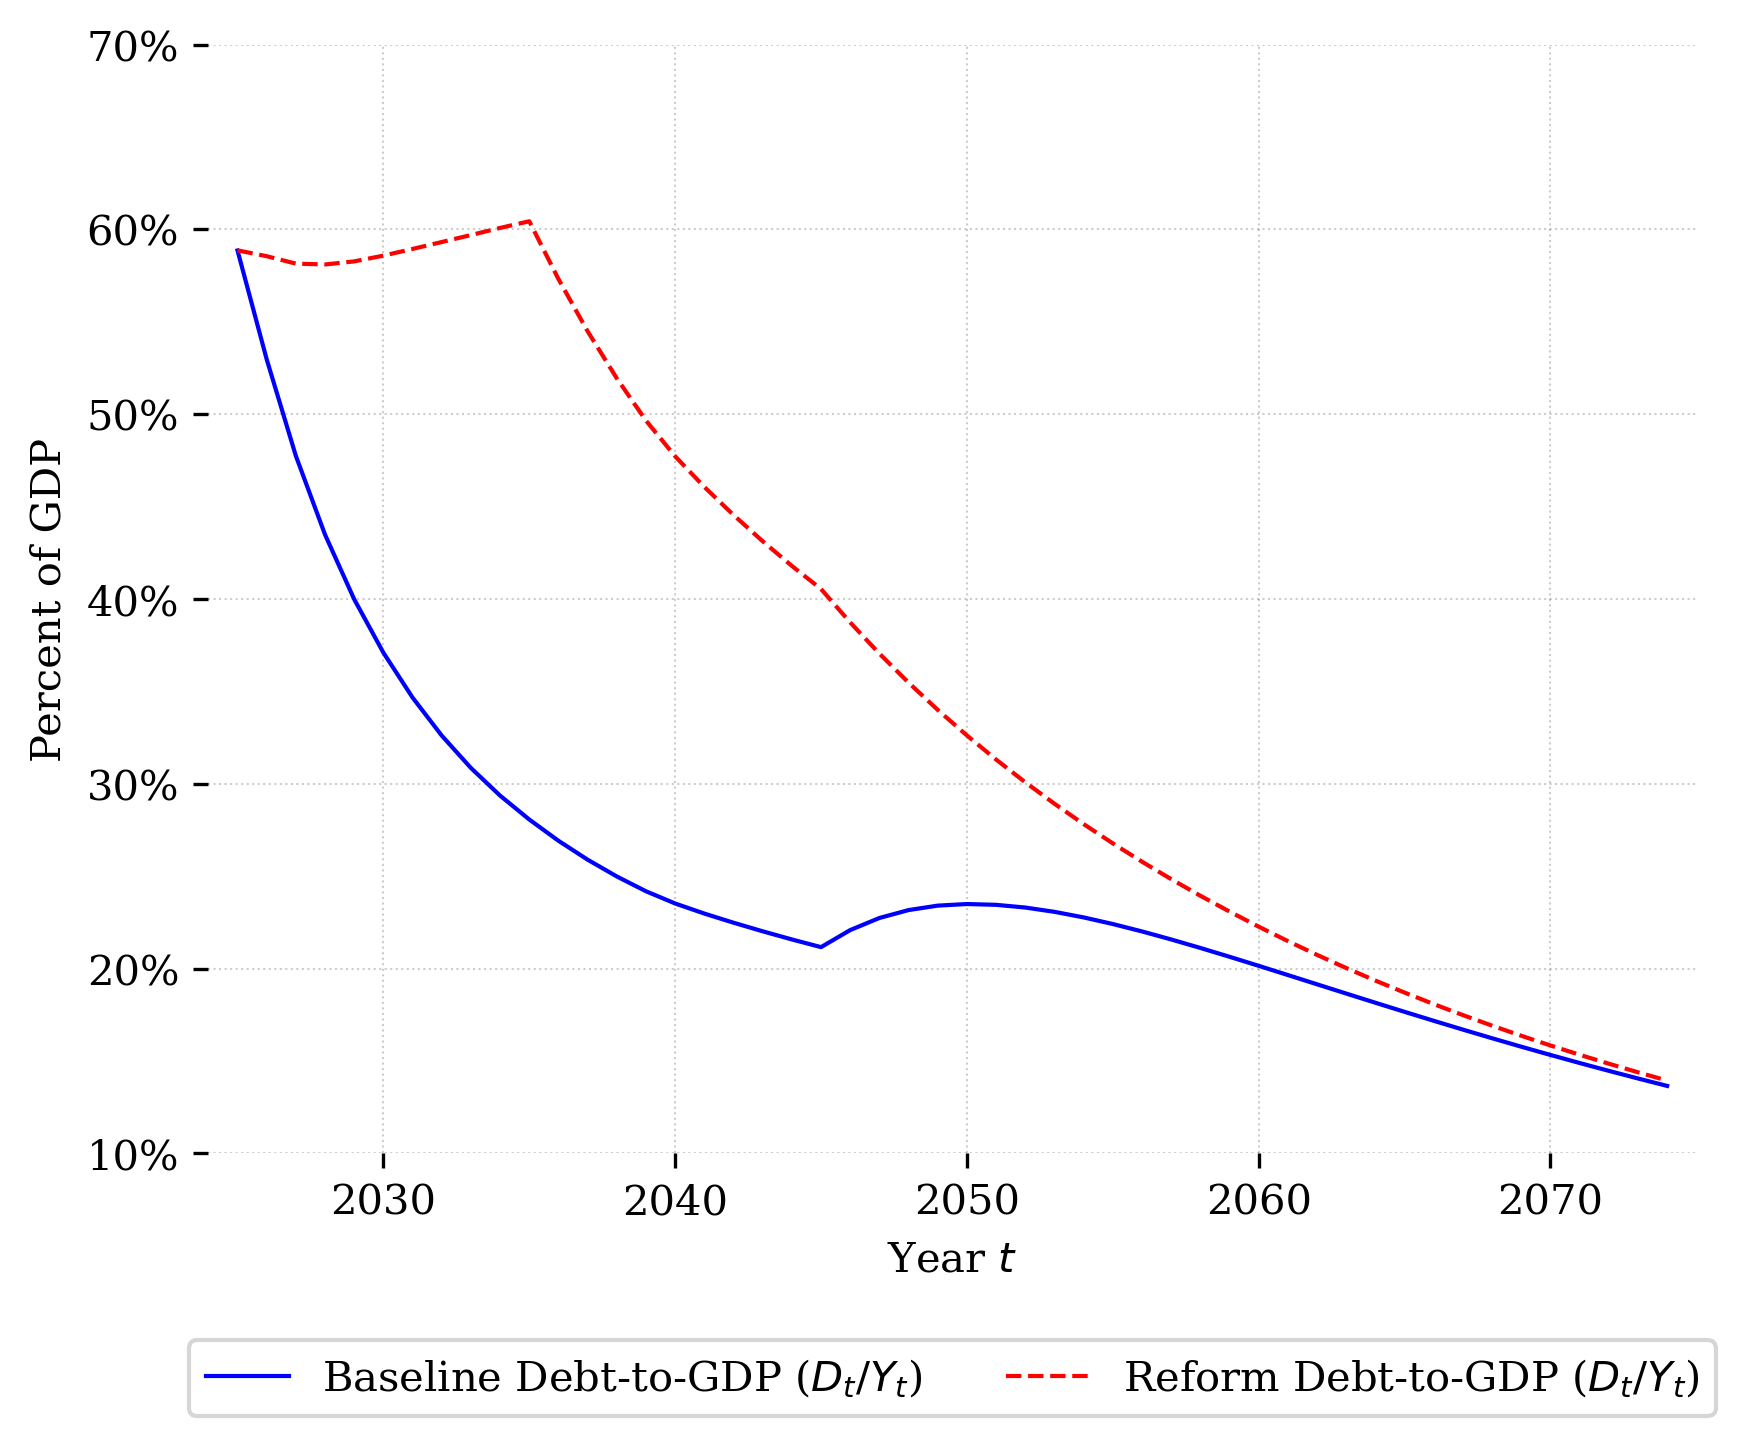
\includegraphics[height=0.75\textheight]{./images/PEP_D_over_Y.png}
  \end{figure}
\end{frame}

\begin{frame}

\frametitle{Long run revenue effects}
\begin{table}
% \caption{NPV of Tax Revenue Effects under Different Discount Rates}
\label{tab:PEP_NPV_Tax_Revenue_Effects_Table}
\begin{tabular}{lrr}
\toprule
 Discount Rate & NPV of Tax Revenue Increase \\
 e & (Trillions PHP) \\
\midrule
 1\% & 294.667 \\
 2\% & 131.213 \\
 3\% & 60.710 \\
 4\% & 29.408 \\
 5\% & 15.041 \\
\bottomrule
\end{tabular}
\end{table}

Note: PEP23 Estimate of government costs: ~2.6-4.2 Trillion PHP

\end{frame}


\section{Dist. Impacts}

\begin{frame}
  \frametitle{Percentage Change in Consumption Good Prices}

  \begin{figure}[htb]\centering
    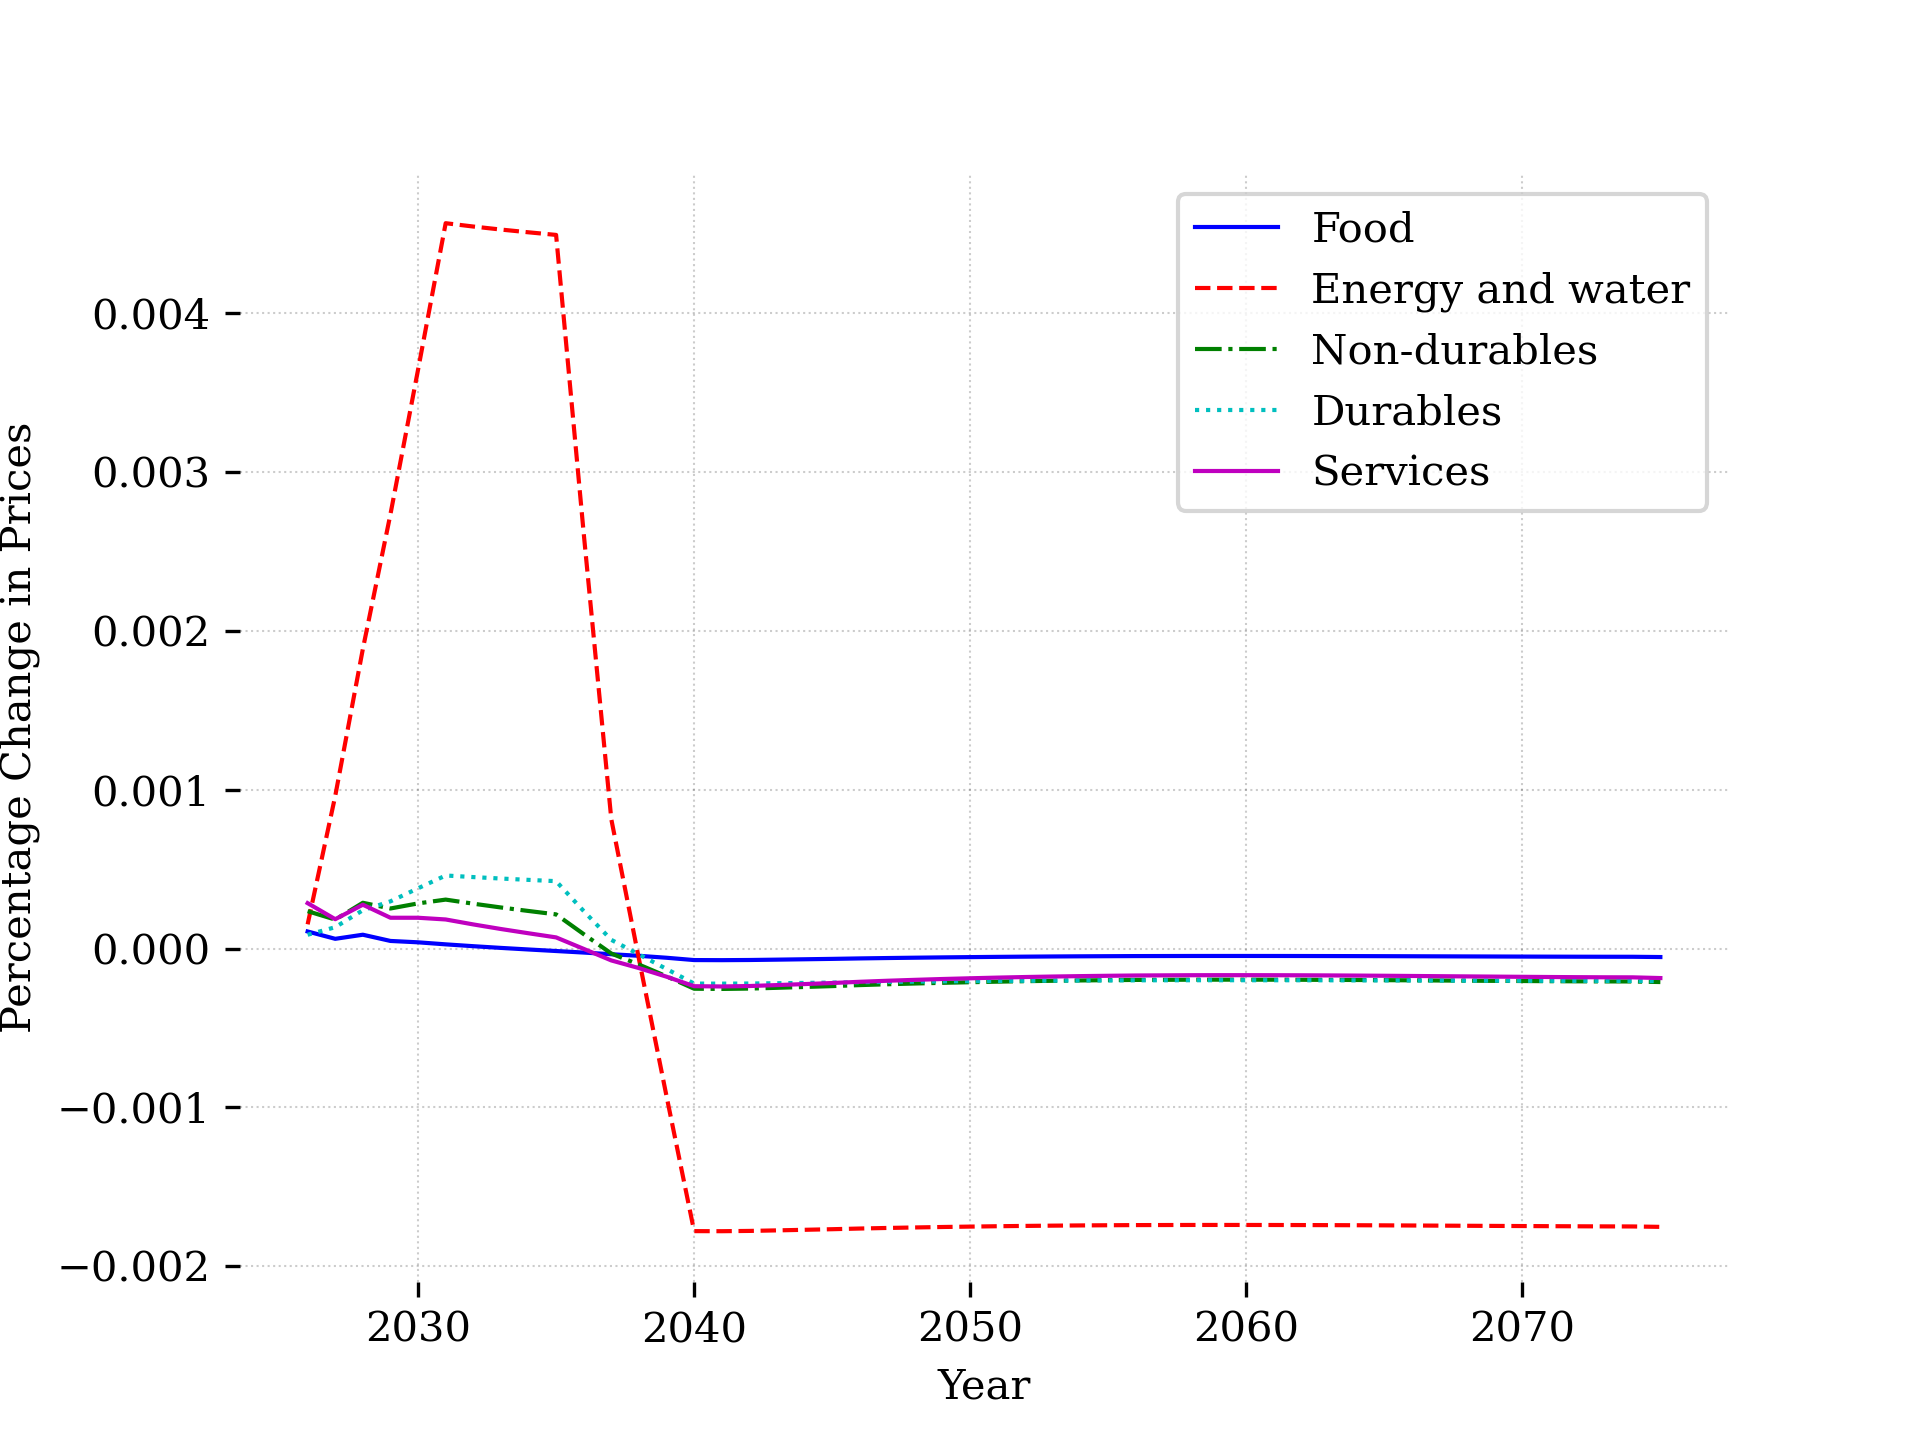
\includegraphics[height=0.75\textheight]{./images/pct_change_p_i.png}
  \end{figure}
\end{frame}


\begin{frame}
  \frametitle{Percentage Change in Production Good Prices}

  \begin{figure}[htb]\centering
    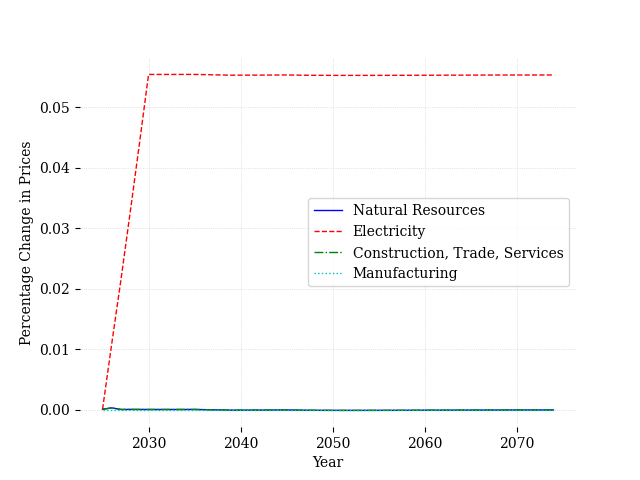
\includegraphics[height=0.75\textheight]{./images/pct_change_p_m.png}
  \end{figure}
\end{frame}


\begin{frame}
  \frametitle{Percentage Change in Consumption Good Prices}

  \begin{figure}[htb]\centering
    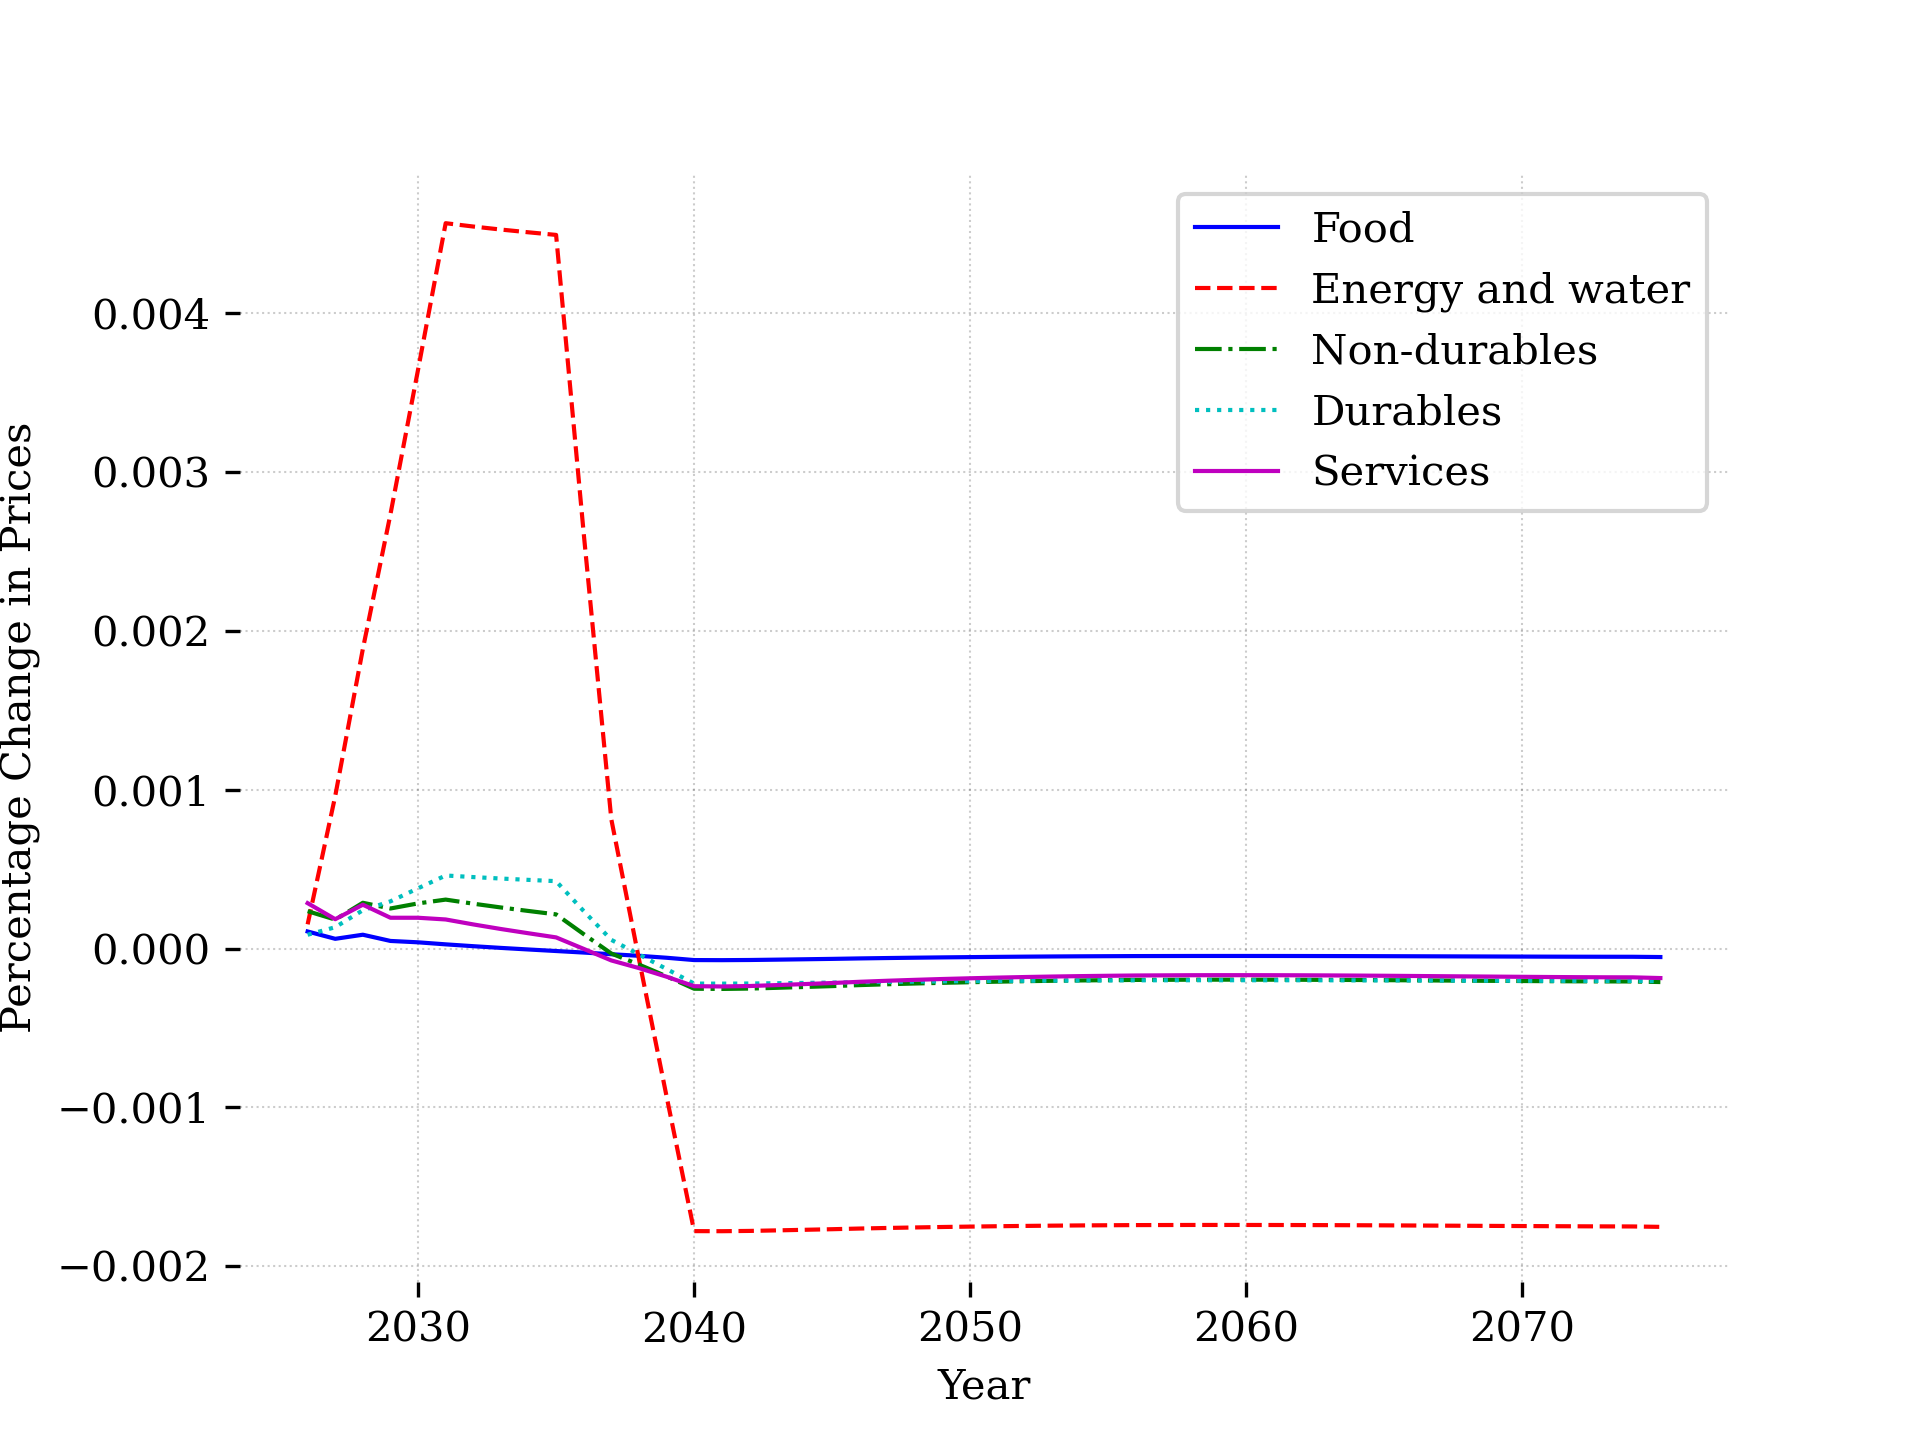
\includegraphics[height=0.75\textheight]{./images/pct_change_p_i.png}
  \end{figure}
\end{frame}


% \begin{frame}
%   \frametitle{Price of Electricity}

%   \begin{figure}[htb]\centering
%     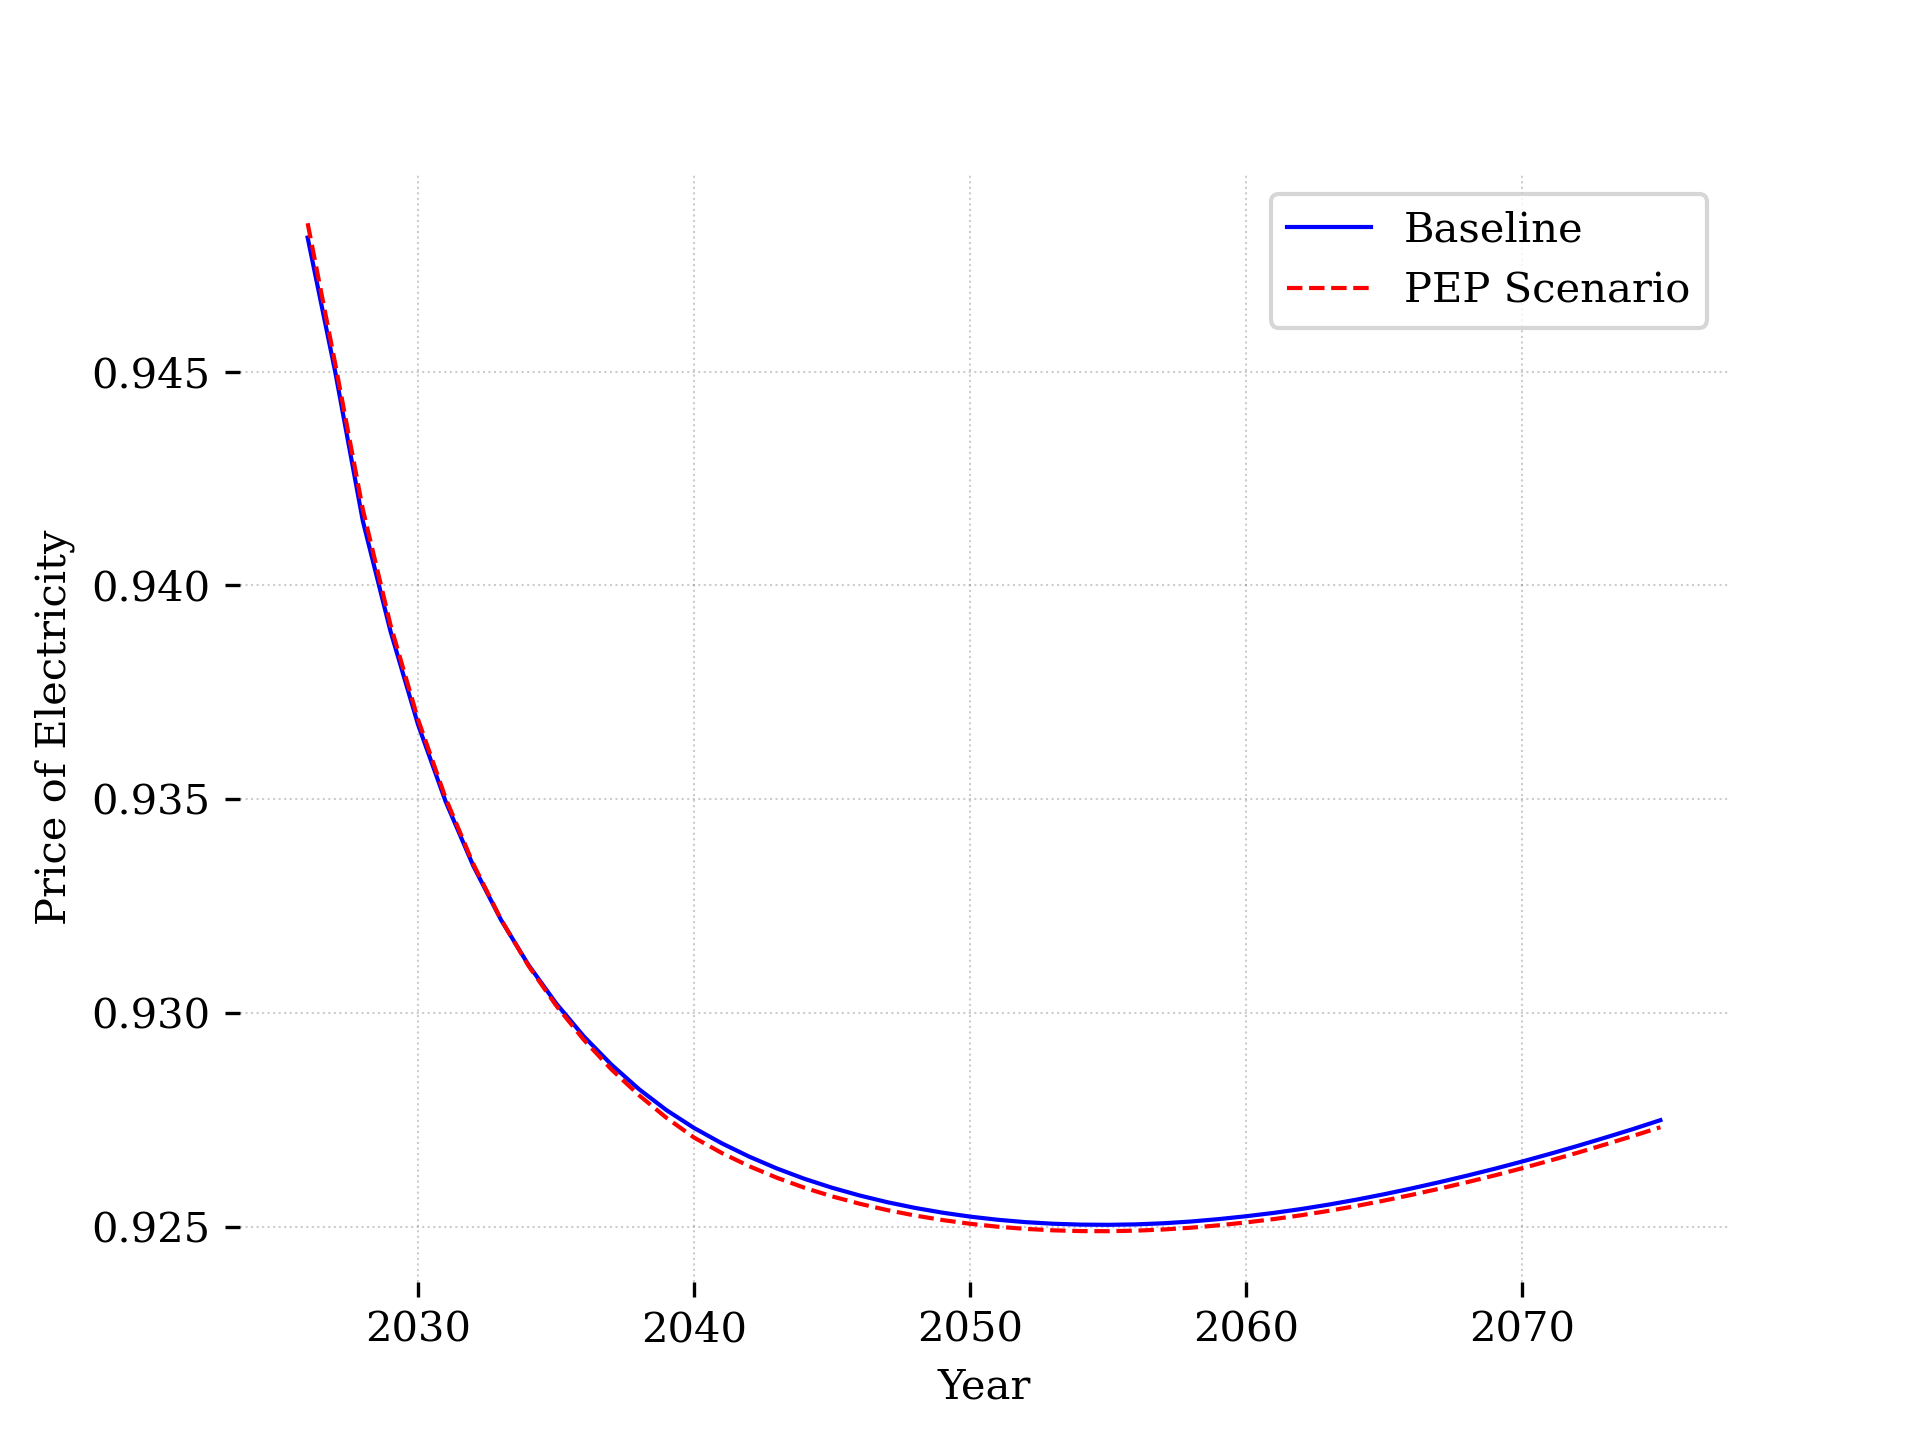
\includegraphics[height=0.75\textheight]{./images/price_of_electricity_plot.png}
%   \end{figure}
% \end{frame}


\begin{frame}
  \frametitle{Percentage Change in Labor Supply by Ability Group}

  \begin{itemize}
    \item Changes over 2036-2046
  \end{itemize}

  \begin{figure}[htb]\centering
    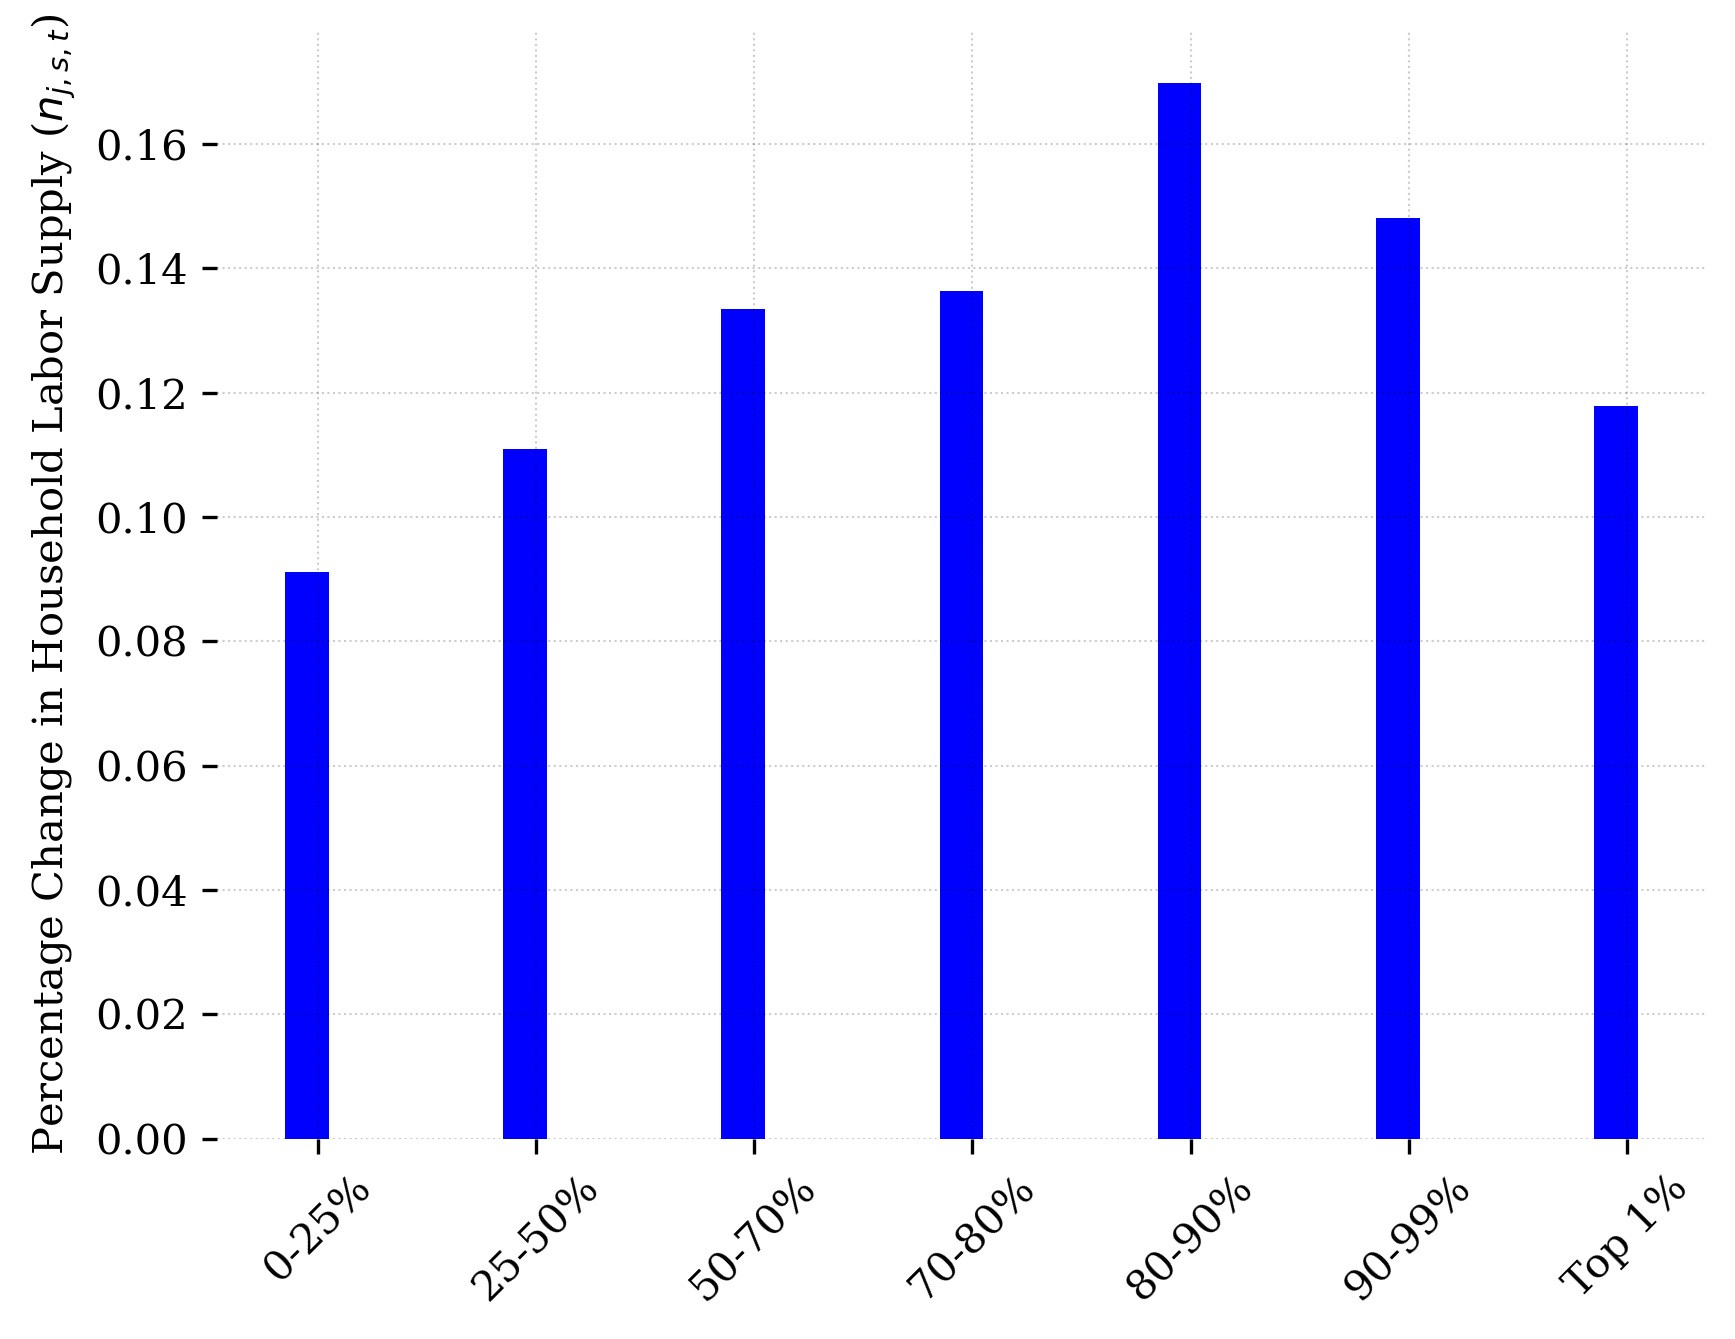
\includegraphics[height=0.65\textheight]{./images/pct_change_n_by_J.png}
  \end{figure}
\end{frame}


\begin{frame}
  \frametitle{Percentage Change in Income by Ability Group}

  \begin{itemize}
    \item Changes over 2036-2046
  \end{itemize}

  \begin{figure}[htb]\centering
    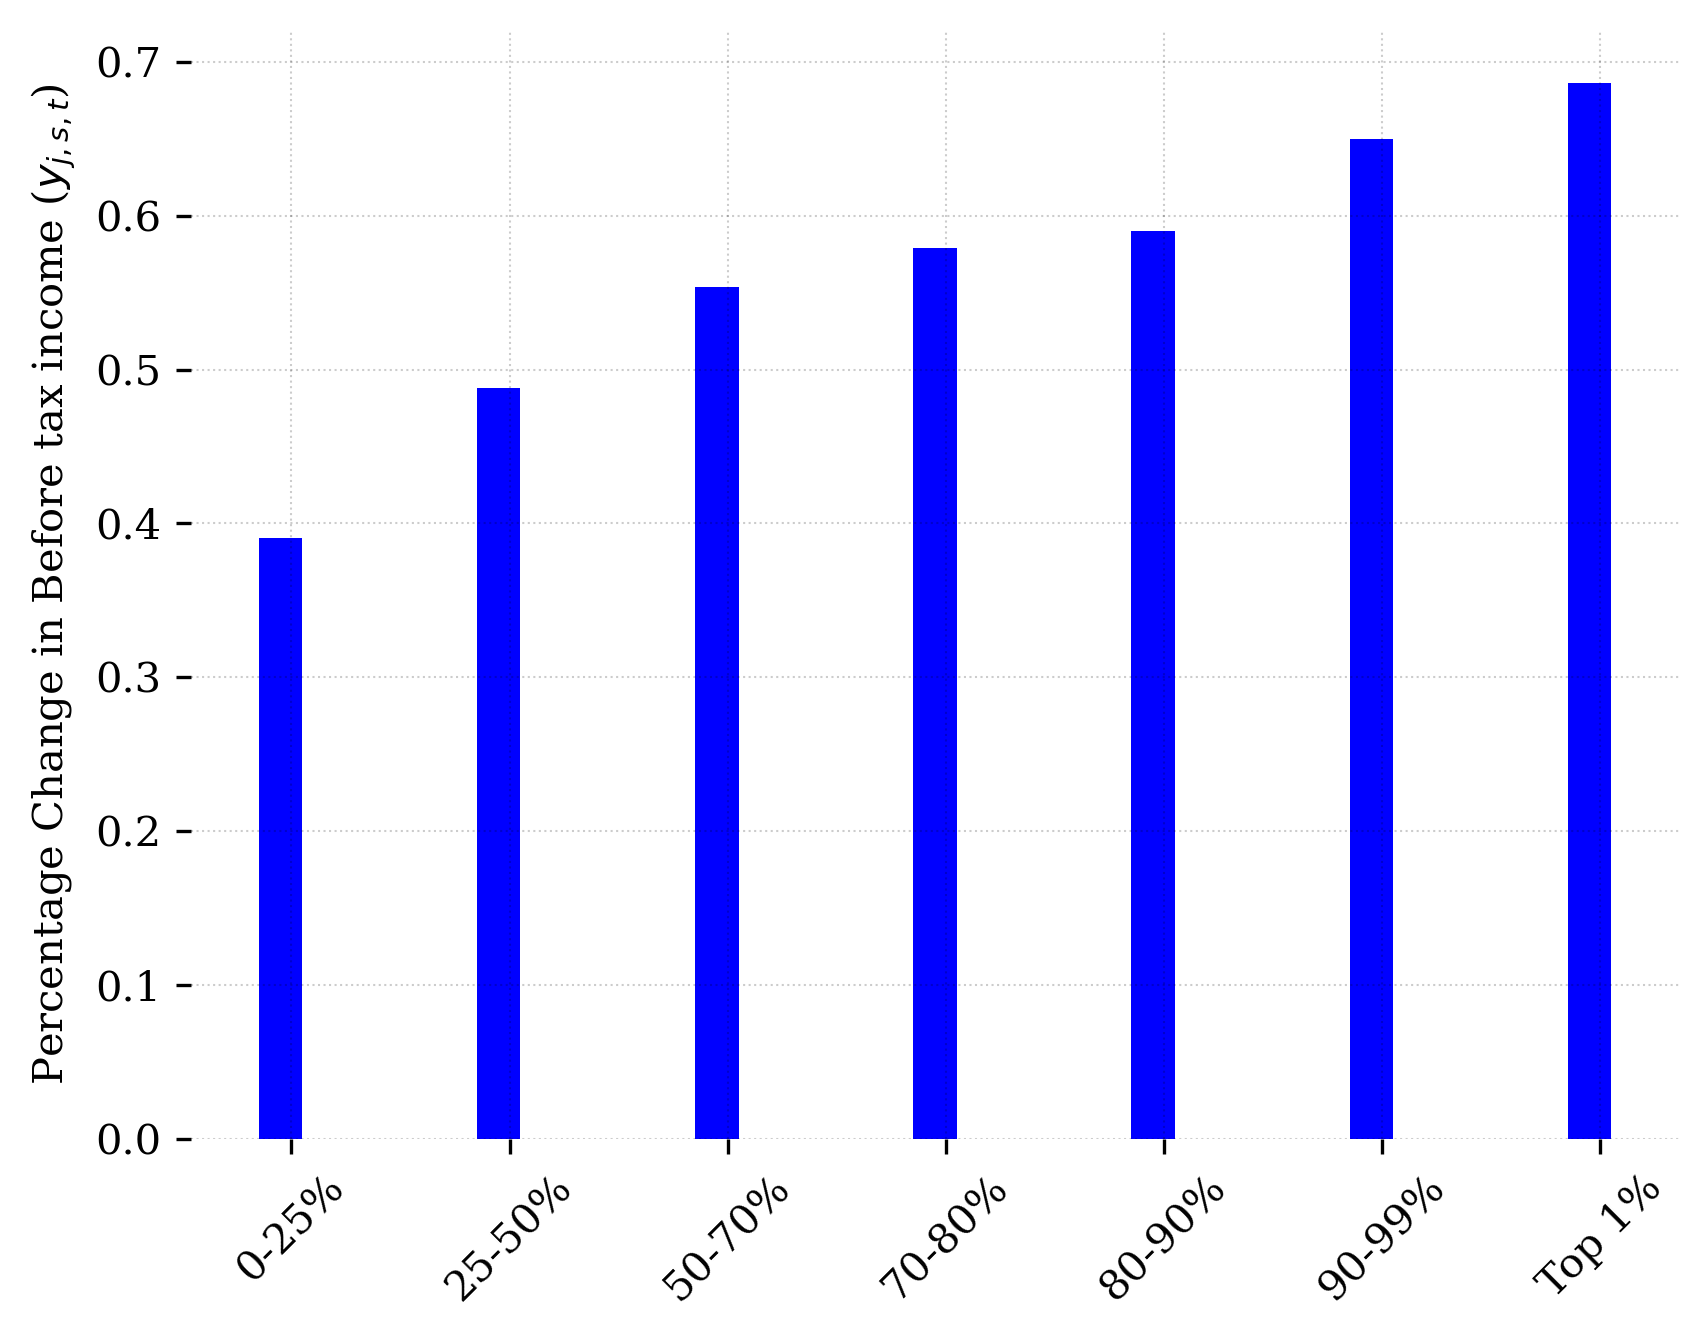
\includegraphics[height=0.65\textheight]{./images/pct_change_before_tax_income_by_J.png}
  \end{figure}
\end{frame}


\begin{frame}
  \frametitle{Percentage Change in Consumption by Ability Group}

  \begin{itemize}
    \item Changes over 2036-2046
  \end{itemize}

  \begin{figure}[htb]\centering
    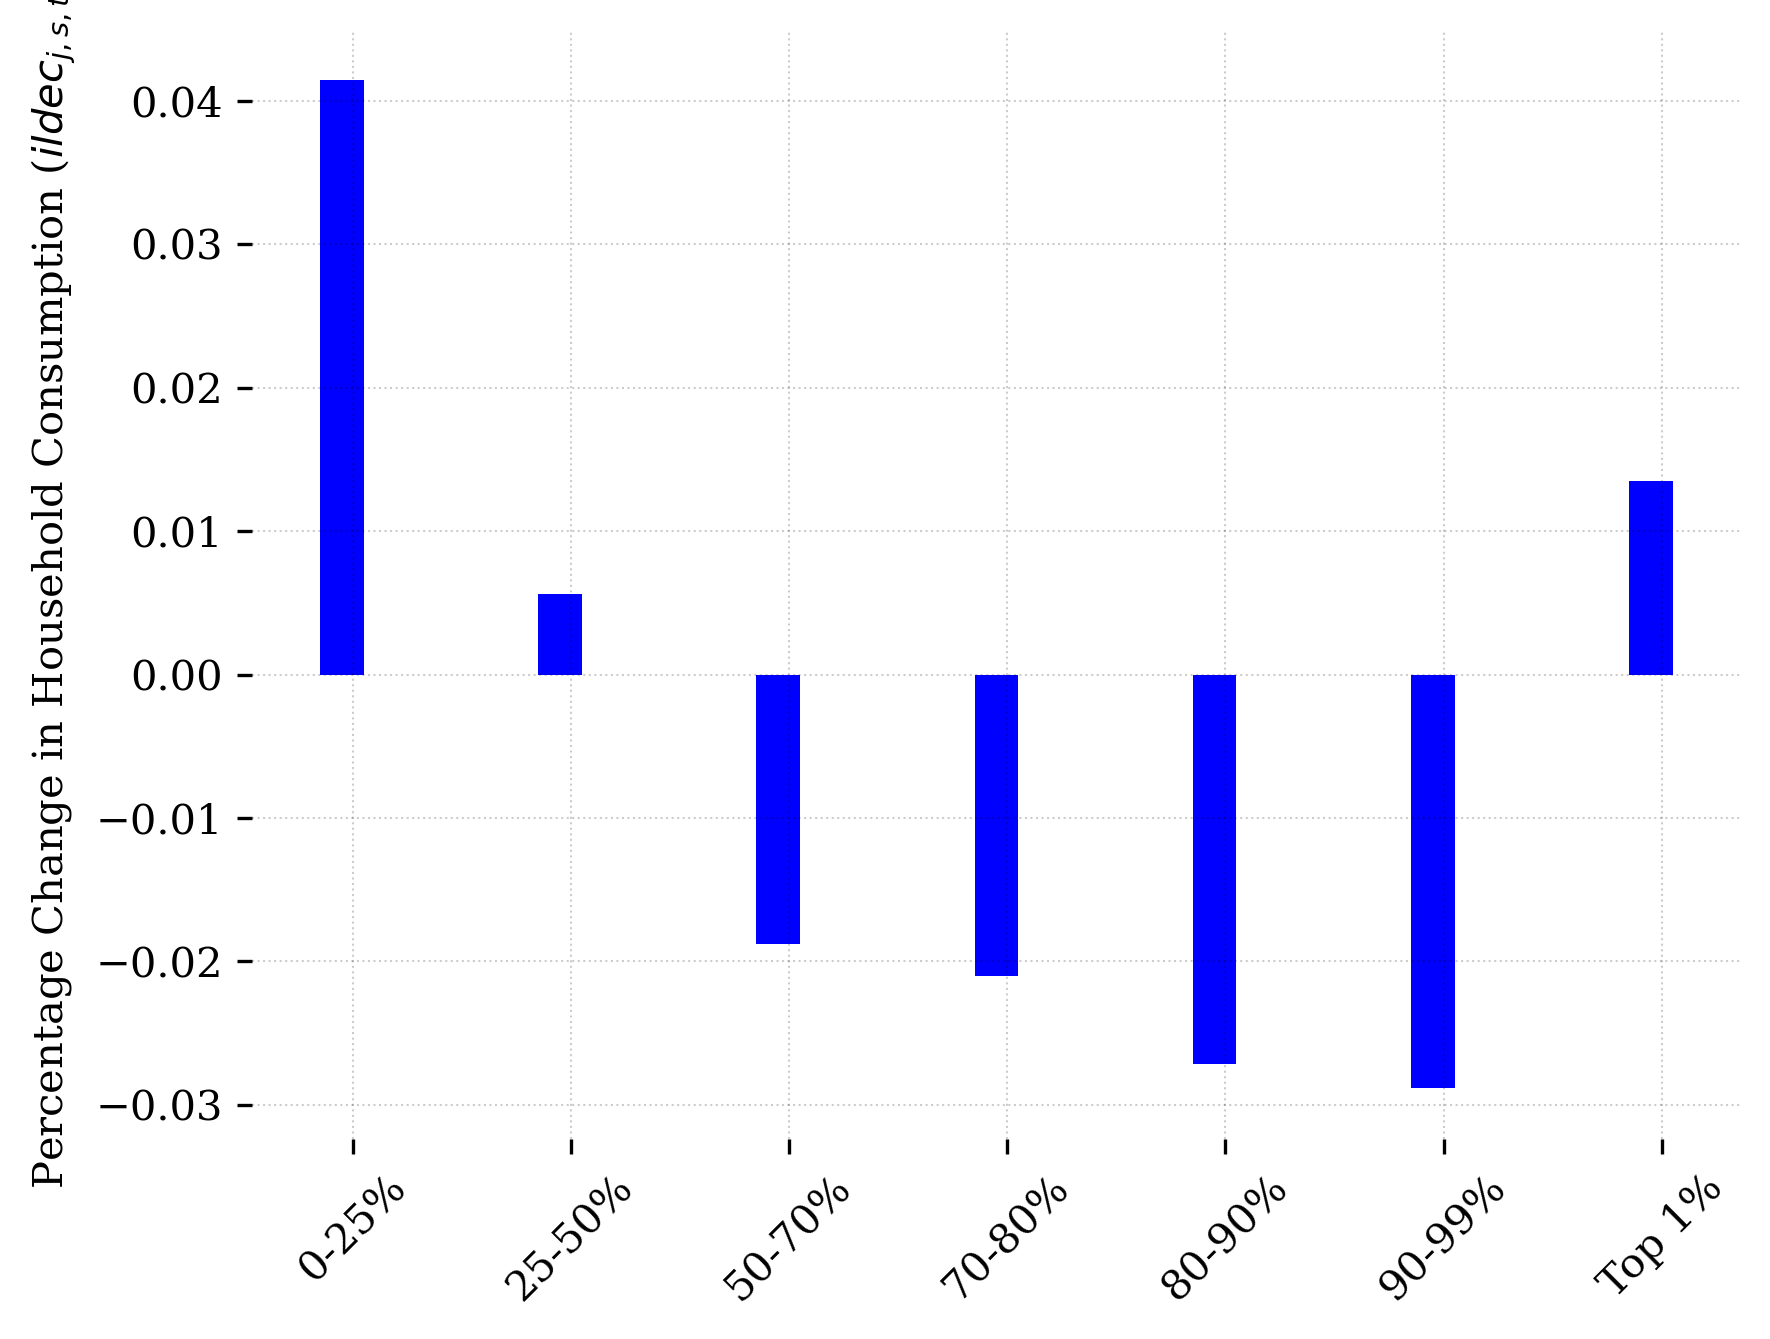
\includegraphics[height=0.65\textheight]{./images/pct_change_c_by_J.png}
  \end{figure}
\end{frame}


\section{Summary}

\begin{frame}
  \frametitle{Key Findings}

  \begin{itemize}
    \item Energy Transition:
      \begin{itemize}
        \item PEP scenario shows increased energy sector TFP over time
        \item Lower electricity generation costs in PEP scenario
        \item Significant upfront investments required
      \end{itemize}
    \item Environmental Benefits:
      \begin{itemize}
        \item Reduced CO2e emissions
        \item Lower PM2.5 concentrations
      \end{itemize}
    \item Health Impacts:
      \begin{itemize}
        \item Improved survival rates and lower mortality
        \item Substantial cumulative deaths averted
        \item Increased labor supply due to better health
      \end{itemize}
  \end{itemize}
\end{frame}


\begin{frame}
  \frametitle{Key Findings (continued)}

  \begin{itemize}
    \item Macroeconomic Effects:
      \begin{itemize}
        \item Positive impacts on capital, output, consumption, and labor
      \end{itemize}
    \item Fiscal Implications:
      \begin{itemize}
        \item Government spending increases for energy investments
        \item Changes in debt-to-GDP ratio
      \end{itemize}
    \item Distributional Effects:
      \begin{itemize}
        \item Changes in relative prices across sectors
        \item Electricity prices adjust over time
        \item Differential impacts across ability groups
      \end{itemize}
  \end{itemize}
\end{frame}


\end{document}
